\SGAchapter{I}{导出范畴中有限性条件的一般理论}{Généralités sur les conditions de finitude dans les catégories dérivées}
\begin{center}L. Illusie\end{center}
\SourcePage{88}
\SGAsection{0}{引言}
第 I 至 IV 讲旨在以适合本讨论班的\Term{generic}{一般}性，发展\Term{ringed-topos}{赋环拓扑斯}的\Term{derived-category}{导出范畴}中\Term{finiteness-condition}{有限性条件}的\Term{form}{形式}体系。
如第 0 讲所说，为了在任意\Term{scheme}{概形}上定义具有良好\Term{variance}{变性}性质的“Grothendieck 群”，我们不得不推广并放宽迄今使用的\Term{finiteness}{有限性}概念。
在\Term{ringed-space}{赋环空间} $(X,\mathcal O_X)$ 上，\Term{coherent-sheaf}{凝聚层}这样的经典概念，一旦 $\mathcal O_X$ 不再\Term{coherent}{凝聚}，就失去了意义。可以考虑用\Term{finite-presentation}{有限表示}来代替，但它有一个缺点：\Term{finite-presentation}{有限表示}模之间的\Term{epimorphism}{满态射}的核，\Term{generic}{一般}不再\Term{finite-presentation}{有限表示}。注意到当 $\mathcal O_X$ \Term{coherent}{凝聚}时，\Term{coherent-sheaf}{凝聚层} $F$ 不仅\Term{finite-presentation}{有限表示}，而且对所有 $n\in\mathbb N$ 都是 $n$ 次\Term{finite-presentation}{有限表示}的，就得到一个满意的概念。所谓“$n$ 次\Term{finite-presentation}{有限表示}”，是指\Term{local-scheme}{局部}存在\Term{exact-sequence}{正合列}
\SourcePage{89}
\[L_n\longrightarrow L_{n-1}\longrightarrow\cdots\longrightarrow L_0\longrightarrow F\longrightarrow0,\]
其中 $L_i$ 是\Term{finite-free}{有限型自由模}。不再假设层 $\mathcal O_X$ \Term{coherent}{凝聚}；若一个 $\mathcal O_X$ 模 $F$ 满足上述条件，即对每个 $n$ 都是 $n$ 次\Term{finite-presentation}{有限表示}的，就称它\Term{pseudo-coherent}{伪凝聚}。这样，\Term{pseudo-coherent}{伪凝聚}性对于\Term{short-exact-sequence}{短正合列}具有和\Term{coherent}{凝聚}性相同的\Term{stable}{稳定}性：若一个 $\mathcal O_X$ 模\Term{short-exact-sequence}{短正合列}的三项中有两项\Term{pseudo-coherent}{伪凝聚}，则第三项也\Term{pseudo-coherent}{伪凝聚}。
这个概念容易推广到层的\Term{complex}{复形}。一个 $\mathcal O_X$ 模\Term{complex}{复形} $F$ 称为\Term{pseudo-coherent}{伪凝聚}的，如果对每个 $n\in\mathbb Z$ 都是 $n$ \Term{pseudo-coherent}{伪凝聚}的；“$n$ \Term{pseudo-coherent}{伪凝聚}”意指\Term{local-scheme}{局部}存在\Term{quasi-isomorphism}{拟同构} $L\to F$，其中 $L$ 是\Term{degree}{次数}\Term{bounded-above}{上有界}的\Term{complex}{复形}，且\Term{degree}{次数} $\geq n$ 的各\Term{set-component}{分量}为\Term{finite-free}{有限型自由模}。对集中于\Term{degree}{次数} $0$ 的\Term{complex}{复形} $F$，作为\Term{complex}{复形}\Term{pseudo-coherent}{伪凝聚}和作为模\Term{pseudo-coherent}{伪凝聚}是一回事。
\Term{pseudo-coherent}{伪凝聚}\Term{complex}{复形}的概念具有出色的\Term{stable}{稳定}性质，第 I 讲第 1、2 节将予以说明。首先，它在 $\mathcal O_X$ \Term{module-category}{模范畴}的\Term{derived-category}{导出范畴} $D(X)$ 中对\Term{isomorphism}{同构}\Term{stable}{稳定}；更进一步，若 $D(X)$ 的一个\Term{distinguished-triangle}{可区别三角形}中两项\Term{pseudo-coherent}{伪凝聚}，则第三项也\Term{pseudo-coherent}{伪凝聚}。换言之，由\Term{pseudo-coherent}{伪凝聚}\Term{complex}{复形}组成的 $D(X)$ 的\Term{full-subcategory}{满子范畴} $D(X)_{\mathrm{coh}}$ 是\Term{triangulated-category}{三角范畴}的\Term{subcategory}{子范畴}。此外，\Term{derive}{导出}\Term{inverse-image}{逆像}和\Term{derive}{导出}\Term{tensor-product}{张量积}保持\Term{pseudo-coherent}{伪凝聚}性。当 $\mathcal O_X$ \Term{coherent}{凝聚}时，\Term{complex}{复形} $F$ \Term{pseudo-coherent}{伪凝聚}恰好表示 $F$ 的\Term{cohomology}{上同调}\Term{local-scheme}{局部}\Term{bounded-above}{上有界}，且所有 $\mathcal H^i(F)$ \Term{coherent}{凝聚}。
若 $\mathcal O_X$ 是\Term{regular}{正则}\Term{local-ring}{局部环}层，则任意\Term{coherent}{凝聚} $\mathcal O_X$ 模 $F$
\SourcePage{90}
\Term{local-scheme}{局部}都有由\Term{finite-free}{有限型自由模}组成的\Term{finite}{有限}左\Term{resolution}{消解}，即\Term{local-scheme}{局部}存在\Term{exact-sequence}{正合列}
\[0\longrightarrow L_n\longrightarrow\cdots\longrightarrow L_0\longrightarrow F\longrightarrow0,\]
其中 $L_i$ 为\Term{finite-free}{有限型自由模}。因此，当 $\mathcal O_X$ 是任意\Term{local-ring}{局部环}层时，自然要研究具有上述性质的模。这样的模称为\Term{perfect-complex}{完美}的。更\Term{generic}{一般}地，一个 $\mathcal O_X$ 模\Term{complex}{复形} $F$ 称为\Term{perfect-complex}{完美}的，如果\Term{local-scheme}{局部}存在\Term{quasi-isomorphism}{拟同构} $L\to F$，其中 $L$ 的\Term{degree}{次数}\Term{bounded}{有界}且各\Term{set-component}{分量}为\Term{finite-free}{有限型自由模}。第 I 讲第 3 节将证明，由\Term{perfect-complex}{完美}\Term{complex}{复形}组成的 $D(X)$ 的\Term{full-subcategory}{满子范畴} $D(X)_{\mathrm{parf}}$ 和 $D(X)_{\mathrm{coh}}$ 一样，是\Term{triangulated-subcategory}{三角子范畴}，并对\Term{derive}{导出}\Term{inverse-image}{逆像}和\Term{derive}{导出}\Term{tensor-product}{张量积}“\Term{stable}{稳定}”。显然 $D(X)_{\mathrm{parf}}\subset D(X)_{\mathrm{coh}}$，但此包含\Term{generic}{一般}是严格的。
可以从\Term{perfect-complex}{完美}性通过“取\Term{limit}{极限}”重新定义\Term{pseudo-coherent}{伪凝聚}性：\Term{complex}{复形} $F$ \Term{pseudo-coherent}{伪凝聚}，当且仅当对任意 $n\in\mathbb Z$，$F$ 都可以“\Term{local-scheme}{局部}以\Term{perfect-complex}{完美}\Term{complex}{复形}作 $n$ 阶逼近”，这意指\Term{local-scheme}{局部}存在\Term{distinguished-triangle}{可区别三角形}
\[\begin{tikzcd} & R\arrow[dl]\arrow[dr] &\\ L\arrow[rr]&&F,\end{tikzcd}\]
其中 $L$ \Term{perfect-complex}{完美}，$R$ 在\Term{degree}{次数} $\geq n$ 无\Term{cohomology}{上同调}。反过来，借助一个附加的\Term{regularity}{正则性}条件，可以从\Term{pseudo-coherent}{伪凝聚}性恢复\Term{perfect-complex}{完美}性：\Term{complex}{复形}\Term{perfect-complex}{完美}，当且仅当它\Term{pseudo-coherent}{伪凝聚}且\Term{local-scheme}{局部}有\Term{finite}{有限}的 \Term{tor-dimension}{Tor 维数}（第 I 讲第 5 节）。由此重新得到：若各\Term{local-ring}{局部环}\Term{regular}{正则}，则每个\Term{coherent-sheaf}{凝聚层}都是\Term{perfect-complex}{完美}的；更\Term{generic}{一般}地，每个\Term{cohomology}{上同调}\Term{local-scheme}{局部}\Term{bounded}{有界}的\Term{pseudo-coherent}{伪凝聚}\Term{complex}{复形}都是\Term{perfect-complex}{完美}的。
\SourcePage{91}
\Term{pseudo-coherent}{伪凝聚}性和\Term{perfect-complex}{完美}性是本讨论班使用的两个基本\Term{finiteness}{有限性}概念。第 I 讲第 1 至 5 节专门给出其定义，建立其初等\Term{stable}{稳定}性质。为此只需\Term{finite-free}{有限型自由模}\Term{category}{范畴}相对于全体\Term{module-category}{模范畴}的两三个\Term{local-nature}{局部性质}。因此，把这种情形公理化就显得方便，而且特别对第 II 讲有用：在一个\Term{site}{景}上的\Term{fibered-category}{纤维范畴}中，相对于满足适当条件的\Term{fibered-subcategory}{纤维子范畴}，引入\Term{pseudo-coherent}{伪凝聚}性（以及\Term{perfect-complex}{完美}性）的概念。
第 I 讲第 6 至 8 节把\Term{finite-type}{有限型}\Term{locally-free}{局部自由}层的一些熟知概念推广到\Term{perfect-complex}{完美}\Term{complex}{复形}：秩、\Term{duality}{对偶性}以及\Term{endomorphism}{自同态}的迹。
第 II 讲讨论“整体\Term{resolution}{消解}的存在性”：在\Term{ringed-topos}{赋环拓扑斯} $(X,\mathcal O_X)$ 上，什么条件下一个\Term{pseudo-coherent}{伪凝聚}（或\Term{perfect-complex}{完美}）\Term{complex}{复形}在 $D(X)$ 中整体\Term{isomorphism}{同构}于一个\Term{finite-type}{有限型}\Term{locally-free}{局部自由}模\Term{complex}{复形}？这个问题的重要性，主要在于目前还不知道如何把\Term{locally-free}{局部自由}模的一些通常构造推广到\Term{perfect-complex}{完美}\Term{complex}{复形}：\Term{exterior-power}{外幂}、\Term{symmetric-power}{对称幂}、\Term{chern-class}{Chern 类}（详情参看第 XIV 讲）。因此，掌握便于运用的整体\Term{resolution}{消解}存在性的充分判据很有用，它能把某些关于\Term{pseudo-coherent}{伪凝聚}（或\Term{perfect-complex}{完美}）\Term{complex}{复形}的问题，化为关于\Term{finite-type}{有限型}\Term{locally-free}{局部自由}层的类似问题。这些判据
\SourcePage{92}
见于第 II 讲。特别证明，下列情形存在整体\Term{resolution}{消解}：$X$ 为\Term{affine}{仿射}\Term{scheme}{概形}的 Zariski \Term{topos}{拓扑斯}；更\Term{generic}{一般}地，$X$ 为具有一个\Term{ample}{丰沛}\Term{invertible-sheaf}{可逆层}，甚至在 Kleiman 意义下具有一族\Term{ample}{丰沛}\Term{invertible-sheaf}{可逆层}的\Term{quasi-compact}{拟紧}\Term{scheme}{概形}的 Zariski \Term{topos}{拓扑斯}（例如一个\Term{regular}{正则}\Term{scheme}{概形}）；或者 $X$ 为紧\Term{topological-space}{拓扑空间}上的\Term{set-sheaf}{集合层}\Term{topos}{拓扑斯}，$\mathcal O_X$ 为复值\Term{continuous}{连续}函数层。为了说明这些概念，并显示它们的灵活性，附录给出一族椭圆\Term{operator}{算子}的指标的一个“纯粹层论的”定义。
第 III 讲研究\Term{finiteness-condition}{有限性条件}在\Term{derive}{导出}\Term{direct-image}{正像}下的\Term{stable}{稳定}性。为了得到合理的陈述，须将\Term{pseudo-coherent}{伪凝聚}性和\Term{perfect-complex}{完美}性的概念“相对化”。这里采用通常\Term{scheme}{概形}的框架，对本讨论班已经足够；不过毫无疑问，迟早必须为相对\Term{scheme}{概形}或\Term{analytic-space}{解析空间}建立类似理论。设 $p:X\to S$ 是\Term{local-scheme}{局部}\Term{finite-type}{有限型}的 $S$ \Term{scheme}{概形}，$F$ 是一个 $\mathcal O_X$ 模\Term{complex}{复形}；若\Term{local-scheme}{局部}可以把 $X$ 通过\Term{closed-immersion}{闭浸入}\Term{embedding}{嵌入}一个\Term{smooth}{光滑} $S$ \Term{scheme}{概形} $X'$，使得 $F$ 在 $X'$ 上的\Term{extension-by-zero}{零延拓}\Term{pseudo-coherent}{伪凝聚}（或\Term{perfect-complex}{完美}），就称 $F$ 相对于 $p$ \Term{pseudo-coherent}{伪凝聚}（或\Term{perfect-complex}{完美}）。相对于 $p$ 的\Term{pseudo-coherent}{伪凝聚}概念，主要在 $S$ 非\Term{locally-noetherian}{局部 Noether} 的情形才有意义，因为在相反情形它和通常的\Term{pseudo-coherent}{伪凝聚}性一致。另一方面，如所预期，$F$ 相对于 $p$ \Term{perfect-complex}{完美}
\SourcePage{93}
\Term{equivalence}{等价}于 $F$ 相对于 $p$ \Term{pseudo-coherent}{伪凝聚}且\Term{local-scheme}{局部}具有\Term{finite}{有限}的相对 \Term{tor-dimension}{Tor 维数}（即相对于\Term{ringed-sheaf}{环层} $p^{-1}(\mathcal O_S)$）。第 III 讲的\Term{center}{中心}\Term{theorem}{定理}是\Term{finiteness-theorem}{有限性定理}，它断言（更精确的\Term{form}{形式}见该讲）：若 $f:X\to Y$ 是\Term{local-scheme}{局部}\Term{finite-type}{有限型} $S$ \Term{scheme}{概形}间的\Term{proper}{固有态射}，则\Term{functor}{函子} $\mathbb Rf_*$ 把相对于 $S$ \Term{pseudo-coherent}{伪凝聚}的\Term{complex}{复形}变成相对于 $S$ \Term{pseudo-coherent}{伪凝聚}的\Term{complex}{复形}。这个\Term{theorem}{定理}实际上还是一个猜想，但下列两个特殊情形已经得到证明：a) $S$ \Term{locally-noetherian}{局部 Noether}；b) $f$ \Term{projective}{射影}。遗憾的是，\Term{generic}{一般}情形的推广似乎与\Term{analytic-geometry}{解析几何}中的类似\Term{theorem}{定理}（Grauert “\Term{theorem}{定理}”）有同等的难度。
将\Term{finiteness-theorem}{有限性定理}与一个本质上平凡的公式，即所谓\Term{projection-formula}{投影公式}结合，可以得到\Term{derive}{导出}\Term{direct-image}{正像}保持相对\Term{perfect-complex}{完美}性的实用判据。作为推论，重新得到“Grauert 的\Term{continuity}{连续性}及\Term{semicontinuity-theorem}{半连续性定理}”（EGA III 7.6）。
第 IV 讲把第 I 至 III 讲的结果翻译成“Grothendieck 群”的语言。在\Term{ringed-topos}{赋环拓扑斯} $(X,\mathcal O_X)$ 上，记 $K^{\boldsymbol\cdot}(X)$（分别 $K_{\boldsymbol\cdot}(X)$）为\Term{perfect-complex}{完美}且具有\Term{finite}{有限} \Term{tor-dimension}{Tor 维数}的\Term{complex}{复形}（分别\Term{pseudo-coherent}{伪凝聚}且\Term{cohomology}{上同调}\Term{bounded}{有界}的\Term{complex}{复形}）\Term{category}{范畴}的“Grothendieck 群”。群 $K^{\boldsymbol\cdot}(X)$ 是一个环，$K_{\boldsymbol\cdot}(X)$ 是其上的模。$K^{\boldsymbol\cdot}$ 是\Term{contravariant-functor}{反变函子}（如上标的点所暗示），而 $K_{\boldsymbol\cdot}$ 对\Term{proper}{固有}且\Term{pseudo-coherent}{伪凝聚}的\Term{morphism}{态射}是\Term{covariant-functor}{协变函子}（\Term{scheme}{概形}或\Term{analytic-space}{解析空间}的\Term{morphism}{态射}，并须以\Term{finiteness-theorem}{有限性定理}可用为前提……）。还有不寻常的\Term{variance}{变性}：
\SourcePage{94}
对于满足适当\Term{regularity}{正则性}假设的\Term{morphism}{态射}，$K^{\boldsymbol\cdot}$ \Term{covariant}{协变}而 $K_{\boldsymbol\cdot}$ \Term{contravariant}{反变}。最后，第 II 讲的整体化判据可以将它们与朴素地从\Term{coherent-sheaf}{凝聚层}或\Term{finite-type}{有限型}\Term{locally-free}{局部自由}层定义的“Grothendieck 群”联系起来。
\SGAsection{1}{预备定义}
\subsection*{1.1. \Term{fiber}{纤维}为\Term{additive-category}{加性范畴}（分别 \Term{abelian-category}{Abel 范畴}、\Term{triangulated-category}{三角范畴}）的\Term{fibre-category}{纤维范畴}}
\textbf{1.1.1.} 设 $\mathscr S$ 为\Term{category}{范畴}，$\mathscr C$ 为一个\Term{fibered-category}{纤维} $\mathscr S$ \Term{category}{范畴}（SGA 1 VI 6.1），各\Term{fiber}{纤维}是\Term{additive-category}{加性范畴}（分别\Term{triangulated-category}{三角范畴}）。若对 $\mathscr S$ 的每个\Term{arrow}{箭头} $f:X\to Y$，\Term{inverse-image}{逆像}\Term{functor}{函子}（在唯一\Term{isomorphism}{同构}意义下确定）$f^*:\mathscr C_Y\to\mathscr C_X$ 是\Term{additive}{加性}的（分别\Term{exact}{正合}的），则称 $\mathscr C$ 是\Term{additive}{加性}（分别三角）$\mathscr S$ \Term{category}{范畴}，或称 $\mathscr C$ 在 $\mathscr S$ 上\Term{additive}{加性}（分别为三角的）。若 $\mathscr C$ 是各\Term{fiber}{纤维}为 \Term{abelian-category}{Abel 范畴}的\Term{additive}{加性} $\mathscr S$ \Term{category}{范畴}，则称它为 Abel $\mathscr S$ \Term{category}{范畴}；若此外各\Term{inverse-image}{逆像}\Term{functor}{函子}\Term{exact}{正合}，则称它为\Term{flat}{平坦} Abel $\mathscr S$ \Term{category}{范畴}。
\textbf{1.1.2.} 设 $\mathscr C$ 是三角 $\mathscr S$ \Term{category}{范畴}。例如，利用 $\mathscr C$ 的一个\Term{cleavage}{劈分}（SGA 1 VI 7.1），可以定义\Term{fiber}{纤维} $\mathscr S$ \Term{category}{范畴} $\operatorname{Tr}(\mathscr C)$，其在每个 $X\in\operatorname{ob}(\mathscr S)$ 上的\Term{fiber}{纤维}，是 $\mathscr C_X$ 中\Term{distinguished-triangle}{可区别三角形}的\Term{category}{范畴} $\operatorname{Tr}(\mathscr C_X)$。
\textbf{1.1.3.} 设 $\mathscr C,\mathscr C'$ 为\Term{additive}{加性}（分别三角）$\mathscr S$ \Term{category}{范畴}，$F:\mathscr C\to\mathscr C'$ 为\Term{functor}{函子}。若 $F$ 是在各\Term{fiber}{纤维}上\Term{additive}{加性}（分别\Term{exact}{正合}）的\Term{cartesian}{笛卡尔} $\mathscr S$ \Term{functor}{函子}，则称 $F$ 为\Term{additive}{加性}（分别\Term{exact}{正合}）$\mathscr S$ \Term{functor}{函子}。
\SourcePage{95}
若 $\mathscr C,\mathscr C'$ 是三角 $\mathscr S$ \Term{category}{范畴}，$F$ 是\Term{exact}{正合} $\mathscr S$ \Term{functor}{函子}，则 $F$ 确定一个\Term{cartesian}{笛卡尔} $\mathscr S$ \Term{functor}{函子} $\operatorname{Tr}(\mathscr C)\to\operatorname{Tr}(\mathscr C')$。
\textbf{1.1.4.} 设 $\mathscr C$ 是三角 $\mathscr S$ \Term{category}{范畴}，$\mathscr C'$ 是 $\mathscr C$ 的满\Term{fiber}{纤维}子 $\mathscr S$ \Term{category}{范畴}。若对每个 $X\in\operatorname{ob}\mathscr S$，$\mathscr C'_X$ 是 $\mathscr C_X$ 的\Term{triangulated-subcategory}{三角子范畴}（[V] 第 I 章第 1 节 2.3），则称 $\mathscr C'$ 为 $\mathscr C$ 的三角子 $\mathscr S$ \Term{category}{范畴}。
\textbf{1.1.5.} 设 $\mathscr C$ 为\Term{additive}{加性} $\mathscr S$ \Term{category}{范畴}。可以定义（SGA 4 XVII 2.2、2.4）\Term{additive}{加性}（分别三角）$\mathscr S$ \Term{category}{范畴} $C(\mathscr C)$（分别 $K(\mathscr C)$），它在 $X\in\operatorname{ob}\mathscr S$ 上的\Term{fiber}{纤维}为 $\mathscr C_X$ 的\Term{complex}{复形}\footnote{\Term{differential}{微分}的\Term{degree}{次数}为 $+1$。}（分别“精确到\Term{homotopy}{同伦}”的\Term{complex}{复形}）\Term{category}{范畴} $C(\mathscr C_X)$（分别 $K(\mathscr C_X)$）。若 $\mathscr C$ 为\Term{flat}{平坦} Abel $\mathscr S$ \Term{category}{范畴}，则可以定义（同上）三角 $\mathscr S$ \Term{category}{范畴} $D(\mathscr C)$，其在 $X$ 上的\Term{fiber}{纤维}为\Term{derived-category}{导出范畴} $D(\mathscr C_X)$；若 $f:X\to Y$ 为 $\mathscr S$ 的\Term{arrow}{箭头}，以 $f^*:D(\mathscr C_Y)\to D(\mathscr C_X)$ 记\Term{inverse-image}{逆像}\Term{functor}{函子}，它由 $f^*:K(\mathscr C_Y)\to K(\mathscr C_X)$ 直接取商得到\footnote{若 $a\in\operatorname{ob}D(\mathscr C_Y)$（或 $K(\mathscr C_Y)$），常把 $f^*(a)$ 简写成 $a_X$。}。通过通常的\Term{degree}{次数}条件，定义满三角子 $\mathscr S$ \Term{category}{范畴} $K^*(\mathscr C)$（分别 $D^*(\mathscr C)$），其中 $*=+,-,b$。
\textbf{1.2. 术语。} 设 $\mathscr S$ 为\Term{site}{景}，$\mathscr C$ 为\Term{flat}{平坦} Abel $\mathscr S$ \Term{category}{范畴}（1.1），$\mathscr C_0$ 为严格满的\Term{fiber}{纤维}子 $\mathscr S$ \Term{category}{范畴}。
设 $X\in\operatorname{ob}\mathscr S$，$F\in\operatorname{ob}\mathscr C_X$。$\mathscr S_{/X}$ 中使得存在\Term{epimorphism}{满态射} $E\to f^*F$、$E\in\operatorname{ob}\mathscr C_{0U}$ 的\Term{arrow}{箭头} $f:U\to X$ 的\Term{set}{集合}，是 $X$ 上的一个\Term{sieve}{筛}。若这个\Term{sieve}{筛}\Term{covering}{覆盖}，则称 $F$ 为 $\mathscr C_0$ \Term{finite-type}{有限型}的（没有混淆之虞时，简称\Term{finite-type}{有限型}）。
\SourcePage{96}
若满足下述条件，就称 $\mathscr C_0$ 对\Term{epimorphism}{满态射}的核\Term{local-scheme}{局部}\Term{stable}{稳定}：对每个 $X\in\operatorname{ob}\mathscr S$ 和 $\mathscr C_X$ 中每个\Term{epimorphism}{满态射} $u:E\to F$，若 $E,F\in\operatorname{ob}\mathscr C_{0X}$，则 $u$ 的核\Term{local-scheme}{局部}在 $\mathscr C_0$ 中（即 $\mathscr S_{/X}$ 中使 $f^*\operatorname{Ker}(u)\in\operatorname{ob}\mathscr C_{0U}$ 的\Term{arrow}{箭头} $f:U\to X$ 构成 $X$ 的一个\Term{refinement}{加细}）。
把长\Term{exact-sequence}{正合列}按标准方法拆成\Term{short-exact-sequence}{短正合列}，可以看出上述条件\Term{equivalence}{等价}于下述表面上更强的条件：对每个 $X\in\operatorname{ob}\mathscr S$ 和 $\mathscr C_X$ 的每个\Term{exact-sequence}{正合列}
\[0\longrightarrow E^0\longrightarrow E^1\longrightarrow\cdots\longrightarrow E^n\longrightarrow0,\tag{*}\]
若 $E^i\in\operatorname{ob}\mathscr C_{0X}$（$1\leq i\leq n$），则 $E^0$ \Term{local-scheme}{局部}在 $\mathscr C_0$ 中。
若对每个这样的\Term{exact-sequence}{正合列} $(*)$，$E^0$ 都是 $\mathscr C_0$ \Term{finite-type}{有限型}的，则称 $\mathscr C_0$ 对\Term{epimorphism}{满态射}的核\Term{locally-quasi-stable}{局部拟稳定}。
另一方面，若对每个 $X$ 和 $\mathscr C_X$ 的每个\Term{epimorphism}{满态射} $u:E\to F$，只要 $F\in\operatorname{ob}\mathscr C_{0X}$，$u$ 就\Term{local-scheme}{局部}有\Term{section}{截面}，则称 $\mathscr C_0$ 在 $\mathscr C$ 中\Term{local-scheme}{局部}\Term{liftable}{可提升}。其充要条件是：对 $\mathscr C_X$ 中每个图
\[\begin{tikzcd}&H\arrow[d]\\E\arrow[r,"u"]&F,\end{tikzcd}\]
其中 $u$ 为\Term{epimorphism}{满态射}，$H\in\operatorname{ob}\mathscr C_0$，使得存在\Term{commutative-diagram}{交换图}
\[\begin{tikzcd}&H_U\arrow[d]\arrow[dl,"v"']\\E_U\arrow[r,"u_U"]&F_U\end{tikzcd}\]
的 $X$ 上方的 $U$ 构成 $X$ 的一个\Term{refinement}{加细}。
\SourcePage{97}
若下述较弱条件成立，则称 $\mathscr C_0$ 在 $\mathscr C$ 中\Term{local-scheme}{局部}\Term{quasi-liftable}{拟可提升}：对每个 $X\in\operatorname{ob}\mathscr S$ 和 $\mathscr C_X$ 中每个\Term{epimorphism}{满态射} $u:E\to F$，若 $F\in\operatorname{ob}\mathscr C_{0X}$，则使得存在 $v:F'\to f^*E$、$F'\in\operatorname{ob}\mathscr C_{0U}$ 且 $f^*(u)v$ 为\Term{epimorphism}{满态射}的 $f:U\to X$ 构成 $X$ 的一个\Term{refinement}{加细}。
此条件\Term{equivalence}{等价}于：对 $\mathscr C_X$ 中每个图
\[\begin{tikzcd}&H\arrow[d]\\E\arrow[r,"u"]&F,\end{tikzcd}\]
其中 $u$ 为\Term{epimorphism}{满态射}，$H\in\operatorname{ob}\mathscr C_0$，使得存在\Term{commutative-diagram}{交换图}
\[\begin{tikzcd}G\arrow[r,"v"]\arrow[d]&H_U\arrow[d]\\E_U\arrow[r,"u_U"]&F_U\end{tikzcd}\]
且 $G\in\operatorname{ob}\mathscr C_0$、$v$ 为\Term{epimorphism}{满态射}的 $U$ 构成 $X$ 的一个\Term{refinement}{加细}。
若 $\mathscr S$ 是混沌\Term{site}{景}，例如点\Term{site}{景}（一个\Term{object}{对象}、一个\Term{morphism}{态射}），则在上述定义中省略副词“\Term{local-scheme}{局部}”。
\subsection*{1.3. 例子}
a) 设 $\mathscr S$ 为点\Term{site}{景}，$A$ 为环，$\mathscr C$ 为左 $A$ \Term{module-category}{模范畴}。由\Term{finite-type}{有限型}\Term{projective-object}{投射}左 $A$ 模组成的\Term{full-subcategory}{满子范畴} $\mathscr C_0$ 对\Term{epimorphism}{满态射}的核\Term{stable}{稳定}，且在 $\mathscr C$ 中\Term{liftable}{可提升}；一个 $A$ 模是 $\mathscr C_0$ \Term{finite-type}{有限型}的，当且仅当它在通常意义下
\SourcePage{98}
\Term{finite-type}{有限型}。由\Term{finite-type}{有限型} $A$ 模组成的\Term{full-subcategory}{满子范畴} $\mathscr C_1$ 在 $\mathscr C$ 中\Term{quasi-liftable}{拟可提升}（但\Term{generic}{一般}不\Term{liftable}{可提升}）；若 $A$ 为 Noether 环，则 $\mathscr C_1$ 对\Term{epimorphism}{满态射}的核\Term{stable}{稳定}。由\Term{finite-type}{有限型}自由 $A$ 模组成的\Term{full-subcategory}{满子范畴} $\mathscr C'_0$ 在 $\mathscr C$ 中\Term{liftable}{可提升}，且对\Term{epimorphism}{满态射}的核\Term{quasi-stable}{拟稳定}（\Term{generic}{一般}不\Term{stable}{稳定}）。
b) 设 $(S,\mathcal O_S)$ 为\Term{local-ring}{局部环}\Term{ringed-space}{赋环空间}，$\mathscr S$ 为 $S$ 的\Term{open-subset}{开集}\Term{site}{景}，$\mathscr C$ 为\Term{functor}{函子} $U\mapsto(\text{左 }\mathcal O_U\text{ 模范畴})$ 定义的\Term{fiber}{纤维}（甚至\Term{splitting}{分裂}的，见 SGA 1 VI 9）$\mathscr S$ \Term{category}{范畴}；$\mathscr C$ 是\Term{flat}{平坦} Abel $\mathscr S$ \Term{category}{范畴}（1.1）。设 $\mathscr C_0$ 为由 $U\mapsto(\text{有限型自由 }\mathcal O_U\text{ 模范畴})$ 定义的严格满\Term{additive}{加性}子 $\mathscr S$ \Term{category}{范畴}。一个 $\mathcal O_S$ 模 $M$ \Term{local-scheme}{局部} $\mathscr C_0$ \Term{finite-type}{有限型}，当且仅当它在通常意义下\Term{finite-type}{有限型}（EGA $0_{\mathrm I}$ 5.2）。由 EGA $0_{\mathrm I}$ 5.2.7 和 5.4.9，$\mathscr C_0$ 对\Term{epimorphism}{满态射}的核\Term{local-scheme}{局部}\Term{stable}{稳定}，且在 $\mathscr C$ 中\Term{local-scheme}{局部}\Term{liftable}{可提升}。
c) 设 $G$ 为群，$\mathscr S$ 为 $G$ \Term{set}{集合}的\Term{topos}{拓扑斯}（SGA 4 V 3.11），$k$ 为域（视为 $\mathscr S$ 中的\Term{constant}{常值}环），$\mathscr C$ 为\Term{functor}{函子} $U\mapsto(\text{左 }k_U\text{ 模范畴})$ 定义的\Term{splitting}{分裂} $\mathscr S$ \Term{category}{范畴}；它是\Term{flat}{平坦} Abel $\mathscr S$ \Term{category}{范畴}。设 $\mathscr C_0$ 为由 $U\mapsto(\text{有限型自由 }k_U\text{ 模范畴})$ 定义的严格满\Term{additive}{加性}子 $\mathscr S$ \Term{category}{范畴}。由于 $\mathscr S$ 中的\Term{localization}{局部化}\Term{equivalence}{等价}于忘掉 $G$ 的\Term{action}{作用}，显然，一个 $G$-$k$ 模 $M$ \Term{local-scheme}{局部} $\mathscr C_0$ \Term{finite-type}{有限型}，当且仅当它作为 $k$ \Term{vector-space}{向量空间}\Term{finite-dimensional}{有限维}；$\mathscr C_0$ 对\Term{epimorphism}{满态射}的核\Term{local-scheme}{局部}\Term{stable}{稳定}，且在 $\mathscr C$ 中\Term{local-scheme}{局部}\Term{liftable}{可提升}。
将 c) 的“Galois”变体留给读者：$G$ 为 profinite 群，$\mathscr S$ 为 $G$ 在其上\Term{continuous-action}{连续作用}的\Term{set}{集合}组成的\Term{topos}{拓扑斯}。
\SourcePage{99}
实际上，b)、c) 都是下例的特殊情形。
d) 设 $(\mathscr S,\mathcal O_S)$ 为\Term{ringed-topos}{赋环拓扑斯}（参看 SGA 4 IV 2.10）\footnote{这里 $\mathcal O_S$ 是 $\mathscr S$ 中的环，有\Term{identity-element}{单位元}，但不一定交换。}，$\mathscr C$ 为\Term{functor}{函子} $U\mapsto(\text{左 }\mathcal O_U\text{ 模范畴})$ 定义的\Term{splitting}{分裂} $\mathscr S$ \Term{category}{范畴}；它是\Term{flat}{平坦} Abel $\mathscr S$ \Term{category}{范畴}。设 $\mathscr C_0$ 为由 $U\mapsto(\text{有限型自由 }\mathcal O_U\text{ 模范畴})$ 定义的严格满\Term{additive}{加性}子 $\mathscr S$ \Term{category}{范畴}。\Term{local-scheme}{局部} $\mathscr C_0$ \Term{finite-type}{有限型}的 $\mathcal O_S$ 模简称\Term{finite-type}{有限型}。$\mathscr C_0$ 对\Term{epimorphism}{满态射}的核\Term{locally-quasi-stable}{局部拟稳定}，且在 $\mathscr C$ 中\Term{local-scheme}{局部}\Term{liftable}{可提升}，这可由下列\Term{lemma}{引理}得到。
\begin{SGAresult}{\Term{lemma}{引理}}{1.3.1}
设 $P$ 为 $\mathcal O_S$ 模。下列条件\Term{equivalence}{等价}：
(i) $P$ \Term{finite-type}{有限型}，且\Term{functor}{函子} $\mathcal H om(P,\cdot)$ \Term{exact}{正合}；
(ii) $P$ \Term{finite-type}{有限型}，且每个\Term{epimorphism}{满态射} $M\to P$ \Term{local-scheme}{局部}有\Term{section}{截面}；
(iii) $P$ \Term{local-scheme}{局部}是\Term{finite-free}{有限型自由模}的\Term{direct-summand}{直和因子}。
\end{SGAresult}
证明是直接的，留给读者作为练习。
\subsection*{1.4. 一个“延拓”\Term{lemma}{引理}（参看 EGA $0_{\mathrm{III}}$ 11.9.1）}
\begin{SGAresult}{命题}{1.4.1}
设 $\mathscr S$ 为\Term{site}{景}，$\mathscr C$ 为\Term{flat}{平坦} Abel $\mathscr S$ \Term{category}{范畴}（1.1），$\mathscr C_0$ 为 $\mathscr C$ 的严格满\Term{additive}{加性}子 $\mathscr S$ \Term{category}{范畴}；假设 $\mathscr C_0$ 在 $\mathscr C$ 中\Term{local-scheme}{局部}\Term{quasi-liftable}{拟可提升}（1.2）。设 $S\in\operatorname{ob}\mathscr S$，$u:E\to F$ 为 $\mathscr C_S$ 的\Term{complex}{复形}间的零次\Term{morphism}{态射}（\Term{differential}{微分}\Term{degree}{次数}为 $+1$），$G$ 为 $u$ 的锥（参看 [V] 第 I 章第 1 节 2.1），$n\in\mathbb Z$；假设 $H^n(G)$ 是
\SourcePage{100}
$\mathscr C_0$ \Term{finite-type}{有限型}的（1.2）。则满足下述性质 (p) 的 $X\in\operatorname{ob}\mathscr S_{/S}$ 构成 $S$ 的一个\Term{refinement}{加细}。
(p) 存在 $M\in\operatorname{ob}\mathscr C_{0X}$ 及 $\mathscr C_X$ 的\Term{arrow}{箭头}
\[r:M\to Z^{n+1}(E_X)=\operatorname{Ker}(E_X^{n+1}\xrightarrow{d_X^{n+1}}E_X^{n+2}),\qquad s:M\to F_X^n,\]
使得下图为\Term{complex}{复形}\Term{morphism}{态射} $u':E'\to F_X$（即 $d_{F_X}^ns=u_X^{n+1}r$）：
\[\begin{tikzcd}[column sep=large]
\cdots\arrow[r]&E_X^{n-1}\arrow[r,"{\binom{d_{E_X}^{n-1}}0}"]\arrow[d,"u_X^{n-1}"]&E_X^n\oplus M\arrow[r,"{(d_{E_X}^n,r)}"]\arrow[d,"{(u_X^n,s)}"]&E_X^{n+1}\arrow[r]\arrow[d,"u_X^{n+1}"]&\cdots\\
\cdots\arrow[r]&F_X^{n-1}\arrow[r]&F_X^n\arrow[r]&F_X^{n+1}\arrow[r]&\cdots
\end{tikzcd}\]
并且 (i) $H^{n+1}(u')$ 为\Term{monomorphism}{单态射}，且 $\operatorname{Im}H^{n+1}(u')=\operatorname{Im}H^{n+1}(u_X)$；(ii) $H^n(u')$ 为\Term{epimorphism}{满态射}。
\end{SGAresult}
形象地说，在\Term{local-scheme}{局部}只修改 $E$ 和 $u$ 的第 $n$ 次，即向 $E^n$ 添加一个 $\mathscr C_0$ 的\Term{object}{对象}，就能\Term{local-scheme}{局部}使 $H^{n+1}(u)$ \Term{injectivity}{单射}而不改变其像，并使 $H^n(u)$ \Term{surjectivity}{满射}。
\begin{proof}
证明步骤如下：先说明\Term{local-scheme}{局部}可以选取 $r,s$，使 $H^{n+1}(u)$ \Term{injectivity}{单射}；
\SourcePage{101}
再证明关于 $H^n(G)$ 的\Term{finiteness}{有限性}假设仍然保持；最后在第 $n$ 次再作一次\Term{local-scheme}{局部}修正，使 $H^n(u)$ \Term{surjectivity}{满射}。
\Term{cohomology}{上同调}\Term{exact-sequence}{正合列}
\[\cdots\longrightarrow H^n(G)\longrightarrow H^{n+1}(E)\xrightarrow{H^{n+1}(u)}H^{n+1}(F)\longrightarrow\cdots\]
表明 $H^{n+1}(u)$ 的核为 $\mathscr C_0$ \Term{finite-type}{有限型}。换言之，使得存在\Term{exact-sequence}{正合列}
\[M\longrightarrow H^{n+1}(E_X)\xrightarrow{H^{n+1}(u_X)}H^{n+1}(F_X),\qquad M\in\operatorname{ob}\mathscr C_{0X},\]
的 $S$ 上方的 $X$ 构成 $S$ 的\Term{refinement}{加细}。由于 $\mathscr C_0$ 在 $\mathscr C$ 中\Term{local-scheme}{局部}\Term{quasi-liftable}{拟可提升}，还可要求 $M\to H^{n+1}(E_X)$ 经 $Z^{n+1}(E_X)$ \Term{factorization}{分解}为
\[M\xrightarrow r Z^{n+1}(E_X)\longrightarrow H^{n+1}(E_X).\]
按构造，复合\Term{arrow}{箭头}
\[M\xrightarrow{u_X^{n+1}r}Z^{n+1}(F_X)\longrightarrow H^{n+1}(F_X)\]
为零，所以 $u_X^{n+1}r$ 经 $B^{n+1}(F_X)=\operatorname{Im}(F_X^n\xrightarrow{d^n}F_X^{n+1})$ \Term{factorization}{分解}。再用\Term{quasi-liftable}{拟可提升}性，可要求它经 $F_X^n$ \Term{factorization}{分解}为
\[M\xrightarrow s F_X^n\longrightarrow B^{n+1}(F_X)\lhook\joinrel\longrightarrow Z^{n+1}(F_X).\]
直接核对可知按 1.4.1 定义的 $u'$ 是满足 (i) 的\Term{complex}{复形}\Term{morphism}{态射}。
设 $G'$ 为 $u':E'\to F_X$ 的锥。证明 $H^n(G')$ 为 $\mathscr C_0$ \Term{finite-type}{有限型}。由构造有\Term{exact-sequence}{正合列}
\[0\longrightarrow E_X\xrightarrow v E'\longrightarrow M[-n]\longrightarrow0,\]
\SourcePage{102}
且 $u'v=u_X$。比较 $G_X$ 与 $G'$，例如可构成 $K(\mathscr C_X)$ 中的“八面体”：
\[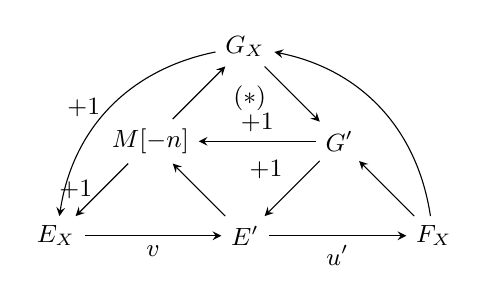
\begin{tikzpicture}[>=stealth,x=1.2cm,y=1.2cm,every node/.style={font=\small}]
\node (G) at (0,2) {$G_X$};
\node (M) at (-1,1) {$M[-n]$};
\node (Gp) at (1,1) {$G'$};
\node (E) at (-2,0) {$E_X$};
\node (Ep) at (0,0) {$E'$};
\node (F) at (2,0) {$F_X$};
\draw[->] (E)--node[below] {$v$}(Ep);
\draw[->] (Ep)--node[below] {$u'$}(F);
\draw[->] (M)--(G);
\draw[->] (G)--(Gp);
\draw[->] (Gp)--node[above] {$+1$}(M);
\draw[->] (M)--node[left] {$+1$}(E);
\draw[->] (Gp)--node[above left] {$+1$}(Ep);
\draw[->] (Ep)--(M);
\draw[->] (F)--(Gp);
\draw[->] (G) to[bend right=35] node[left] {$+1$}(E);
\draw[->] (F) to[bend right=35] (G);
\node at (0.05,1.45) {$(*)$};
\end{tikzpicture}\]
其中三角形 $(*)$ 为 $M[-n]\to G_X\to G'\xrightarrow{+1}M[-n]$。其\Term{cohomology}{上同调}\Term{exact-sequence}{正合列}说明 $H^n(G_X)\to H^n(G')$ \Term{surjectivity}{满射}，因此 $H^n(G')$ 确为 $\mathscr C_0$ \Term{finite-type}{有限型}。
上面的修正把问题归结到 $H^{n+1}(u)$ 是\Term{monomorphism}{单态射}的情形，以下假定如此。$E\to F\to G$ 的\Term{cohomology}{上同调}\Term{exact-sequence}{正合列}给出
\[H^n(E)\xrightarrow{H^n(u)}H^n(F)\longrightarrow H^n(G)\longrightarrow0.\tag{.}\]
由于 $H^n(G)$ 为 $\mathscr C_0$ \Term{finite-type}{有限型}，按定义，使得存在\Term{epimorphism}{满态射} $M\to H^n(G_X)$、$M\in\operatorname{ob}\mathscr C_{0X}$ 的 $X$ 构成 $S$ 的\Term{refinement}{加细}。利用 $\mathscr C_0$ 的\Term{local-scheme}{局部}\Term{quasi-liftable}{拟可提升}性，可要求此\Term{epimorphism}{满态射}经 $Z^n(F_X)$ \Term{factorization}{分解}为
\[M\xrightarrow s Z^n(F_X)\longrightarrow H^n(F_X)\longrightarrow H^n(G_X).\]
显然，取 $r=0$，按 1.4.1 定义的 $u'$ 为\Term{complex}{复形}\Term{morphism}{态射}，且 $H^{n+1}(u')=H^{n+1}(u_X)$。另一方面，由\Term{exact-sequence}{正合列} $(.)$ 立即可见
\SourcePage{103}
\[H^n(u'):H^n(E_X)\oplus M\longrightarrow H^n(F_X)\]
为\Term{epimorphism}{满态射}。这就完成了 1.4.1 的证明。
\end{proof}
\begin{SGAresult}{\Term{lemma}{引理}}{1.4.2}
设 $\mathscr C$ 为 \Term{abelian-category}{Abel 范畴}，$u:E\to F$ 为 $\mathscr C$ 的\Term{complex}{复形}\Term{morphism}{态射}（分别 $D(\mathscr C)$ 的\Term{arrow}{箭头}），$G$ 为 $u$ 的锥。给定 $n\in\mathbb Z$，下列条件\Term{equivalence}{等价}：
(i) 对 $i\geq n$，$H^i(G)=0$；
(ii) $H^i(u)$ 对 $i>n$ 为\Term{isomorphism}{同构}，对 $i=n$ 为\Term{epimorphism}{满态射}。
\end{SGAresult}
由\Term{cohomology}{上同调}\Term{exact-sequence}{正合列}立即得到证明。
\begin{SGAresult}{定义}{1.4.3}
若 $u$ 满足 1.4.2 的\Term{equivalence}{等价}条件，称 $u$ 为 $n$ \Term{quasi-isomorphism}{拟同构}（分别 $n$ \Term{isomorphism}{同构}）。
\end{SGAresult}
由 1.4.1 立即得到：
\begin{SGAresult}{推论}{1.4.4}
设 $\mathscr S,S,\mathscr C,\mathscr C_0$ 如 1.4.1。设 $u:E\to F$ 为 $\mathscr C_S$ 中\Term{complex}{复形}的 $(n+1)$ \Term{quasi-isomorphism}{拟同构}（$n\in\mathbb Z$ 给定），且 $H^n(G)$ 为 $\mathscr C_0$ \Term{finite-type}{有限型}。则使得存在如 1.4.1 的 $(M,r,s)$、使 $u'$ 为 $n$ \Term{quasi-isomorphism}{拟同构}的 $S$ 上方的 $X$ 构成 $S$ 的\Term{refinement}{加细}。
\end{SGAresult}
形象地说，借助 $H^n(G)$ 的\Term{finiteness-condition}{有限性条件}，可以\Term{local-scheme}{局部}“再进一级”：向 $E^n$ 添加一个 $\mathscr C_0$ 的\Term{object}{对象}，在\Term{local-scheme}{局部}修改 $u$ 的第 $n$ 次，使之成为 $n$ \Term{quasi-isomorphism}{拟同构}。
\begin{SGAresult}{推论}{1.4.5}
设 $\mathscr C$ 为 \Term{abelian-category}{Abel 范畴}，$n\in\mathbb Z$，$u:E\to F$ 为 $\mathscr C$ 的\Term{complex}{复形}间的 $n$ \Term{quasi-isomorphism}{拟同构}。存在 $C(\mathscr C)$ 中的\Term{commutative-diagram}{交换图}
\[\begin{tikzcd}E\arrow[r,"v"]\arrow[d,"u"']&E'\arrow[dl,"u'"]\\F&\end{tikzcd}\]
\SourcePage{104}
其中 $u'$ 为\Term{quasi-isomorphism}{拟同构}，$v$ 为\Term{monomorphism}{单态射}，在\Term{degree}{次数} $\geq n$ 诱导\Term{identity-map}{恒等映射}（即对 $i\geq n$，$E'^i=E^i$ 且 $v^i=\operatorname{Id}(E^i)$）。
\end{SGAresult}
\begin{proof}
在 $\mathscr S$ 为点\Term{site}{景}且 $\mathscr C_0=\mathscr C$ 的情形应用 1.4.4，得到 $C(\mathscr C)$ 中的\Term{commutative-triangle}{交换三角形}
\[\begin{tikzcd}E\arrow[r,"v_{n-1}"]\arrow[d,"u"']&E'_{n-1}\arrow[dl,"u'_{n-1}"]\\F&\end{tikzcd}\]
其中 $u'_{n-1}$ 是 $(n-1)$ \Term{quasi-isomorphism}{拟同构}，$v_{n-1}$ 为在\Term{degree}{次数} $\geq n$ 诱导\Term{identity-map}{恒等映射}的\Term{monomorphism}{单态射}。迭代此过程，对 $i\leq n-1$ 得到一列 $C(\mathscr C)$ 中的\Term{commutative-triangle}{交换三角形}
\[\begin{tikzcd}E'_i\arrow[r,"v_{i-1}"]\arrow[d,"u'_i"']&E'_{i-1}\arrow[dl,"u'_{i-1}"]\\F&\end{tikzcd}\]
其中 $u'_i$ 是 $i$ \Term{quasi-isomorphism}{拟同构}，$v_{i-1}$ 是在\Term{degree}{次数} $\geq i$ 诱导\Term{identity-map}{恒等映射}的\Term{monomorphism}{单态射}。取\Term{limit}{极限}即得推论。更精确地，记 $E'_i$ 的\Term{differential}{微分}为 $d'_i$，定义 $E'$ 为
\[E'^i=E^i,\quad d'^i=d^i\quad(i\geq n),\qquad E'^i=(E'_i)^i,\quad d'^i=(d'_i)^i\quad(i<n),\]
再定义 $v,u'$ 为
\[v^j=(v_i)^j,\qquad u'^j=(u'_i)^j\quad(i<j).\]
立即可核对，这样定义的 $E',v,u'$ 满足要求。
\end{proof}
\SourcePage{105}
换言之，简要地说，可以把一个 $n$ \Term{quasi-isomorphism}{拟同构}延拓为\Term{quasi-isomorphism}{拟同构}，“丝毫不改变\Term{degree}{次数} $\geq n$ 已给定的部分”。
\SGAsection{2}{伪凝聚复形}
\textbf{2.0.} 本节中，$\mathscr S$ 表示一个\Term{site}{景}，$S$ 为 $\mathscr S$ 的\Term{object}{对象}，$\mathscr C$ 为\Term{flat}{平坦} Abel $\mathscr S$ \Term{category}{范畴}（1.1），$\mathscr C_0$ 为 $\mathscr C$ 的严格满\Term{additive}{加性}子 $\mathscr S$ \Term{category}{范畴}。假设 $\mathscr C_0$ 对\Term{epimorphism}{满态射}的核\Term{locally-quasi-stable}{局部拟稳定}（1.2），并在 $\mathscr C$ 中\Term{local-scheme}{局部}\Term{quasi-liftable}{拟可提升}（1.2）。
\begin{SGAresult}{定义}{2.1}
设 $X\in\operatorname{ob}\mathscr S$，$E$ 为 $\mathscr C_X$ 的\Term{complex}{复形}，$n\in\mathbb Z$。若对充分大的 $i$ 有 $E^i=0$，并且对 $i\geq n$ 有 $E^i\in\operatorname{ob}\mathscr C_{0X}$，则称 $E$ 严格 $\mathscr C_0$-$n$ \Term{pseudo-coherent}{伪凝聚}；若后一条件对所有 $i$ 成立，则称 $E$ 严格 $\mathscr C_0$ \Term{pseudo-coherent}{伪凝聚}；若此外除\Term{finite}{有限}多个 $i$ 外均有 $E^i=0$，则称 $E$ 严格 $\mathscr C_0$ \Term{perfect-complex}{完美}。
\end{SGAresult}
没有混淆之虞时，有时用“严格 $n$ \Term{pseudo-coherent}{伪凝聚}（分别……）”来代替“严格 $\mathscr C_0$-$n$ \Term{pseudo-coherent}{伪凝聚}（分别……）”。
\begin{SGAresult}{\Term{lemma}{引理}}{2.1.1}
设 $E\in\operatorname{ob}C(\mathscr C_S)$，$n\in\mathbb Z$。若 $E$ 严格 $n$ \Term{pseudo-coherent}{伪凝聚}，且对 $i>n$ 有 $H^i(E)=0$，则 $H^n(E)$ \Term{finite-type}{有限型}。
\end{SGAresult}
\begin{proof}
序列
\[0\longrightarrow Z^n(E)\longrightarrow E^n\longrightarrow E^{n+1}\longrightarrow\cdots\longrightarrow0\]
\Term{exact}{正合}，且对 $i\geq n$ 有 $E^i\in\operatorname{ob}\mathscr C_0$。由于 $\mathscr C_0$ 对\Term{epimorphism}{满态射}的核\Term{locally-quasi-stable}{局部拟稳定}，$Z^n(E)$ \Term{finite-type}{有限型}，因而它的商 $H^n(E)$ 也\Term{finite-type}{有限型}。
\end{proof}
\SourcePage{106}
\begin{SGAresult}{命题}{2.2}
设 $F\in\operatorname{ob}D(\mathscr C_S)$，$n\in\mathbb Z$。则：
a) 若 $F$ 严格 $n$ \Term{pseudo-coherent}{伪凝聚}（相对于 $\mathscr C_0$），且 $u:E\to F$ 为\Term{quasi-isomorphism}{拟同构}，则使得存在\Term{quasi-isomorphism}{拟同构} $v:F'\to E_X$、其中 $F'$ 严格 $n$ \Term{pseudo-coherent}{伪凝聚}的 $S$ 上方的 $X$ 构成 $S$ 的一个\Term{refinement}{加细}。
b) 下列条件\Term{equivalence}{等价}：
(i) 使得存在 $C(\mathscr C_X)$ 中的\Term{quasi-isomorphism}{拟同构} $u:E\to F_X$、且 $E$ 严格 $n$ \Term{pseudo-coherent}{伪凝聚}的 $S$ 上方的 $X$ 构成 $S$ 的一个\Term{refinement}{加细}；
(i$'$) 同 (i)，但 $u$ 为 $D(\mathscr C_X)$ 中的\Term{isomorphism}{同构}；
(ii) 使得存在 $C(\mathscr C_X)$ 中的 $n$ \Term{quasi-isomorphism}{拟同构}（1.4.3）$u:E\to F_X$、且 $E$ 严格\Term{perfect-complex}{完美}的 $S$ 上方的 $X$ 构成 $S$ 的一个\Term{refinement}{加细}；
(ii$'$) 同 (ii)，但 $u$ 为 $D(\mathscr C_X)$ 中的 $n$ \Term{isomorphism}{同构}。
\end{SGAresult}
\begin{proof}
a) 对某个充分大的整数 $i$，存在 $i$ \Term{quasi-isomorphism}{拟同构} $v_i:F'_i\to E$，其中 $F'_i$ 严格 $n$ \Term{pseudo-coherent}{伪凝聚}（取 $F'_i=0$）。证明：若 $i>n$，则\Term{refinement}{加细} $S$ 后，存在 $(i-1)$ \Term{quasi-isomorphism}{拟同构} $v_{i-1}:F'_{i-1}\to E$，其中 $F'_{i-1}$ 严格 $n$ \Term{pseudo-coherent}{伪凝聚}。由 1.4.4，只须证明 $H^{i-1}(M')$ 为 $\mathscr C_0$ \Term{finite-type}{有限型}，其中 $M'$ 是 $v_i$ 的锥。若 $M''$ 为 $uv_i$ 的锥，由 $u$ 是\Term{quasi-isomorphism}{拟同构}及 1.4.2，得到
\[H^j(M')\simeq H^j(M'')\quad\text{对所有 }j,\qquad H^j(M')=0\quad(j\geq i).\]
\SourcePage{107}
另一方面，锥的公式 $M''^j=F_i'^{\,j+1}\oplus F^j$ 表明 $M''$ 严格 $(i-1)$ \Term{pseudo-coherent}{伪凝聚}。故由 2.1.1，$H^{i-1}(M'')=H^{i-1}(M')$ \Term{finite-type}{有限型}，断言得证。迭代并\Term{refinement}{加细} $S$ 后，得到 $n$ \Term{quasi-isomorphism}{拟同构} $v_n:F'_n\to E$，其中 $F'_n$ 严格 $n$ \Term{pseudo-coherent}{伪凝聚}。但由 1.4.5，可以将 $v_n$ 延拓成\Term{quasi-isomorphism}{拟同构} $v:F'\to E$，不改变\Term{degree}{次数} $\geq n$ 的部分，特别使 $F'$ 仍严格 $n$ \Term{pseudo-coherent}{伪凝聚}，a) 得证。
b) 条件 (i) 和 (i$'$) 的\Term{equivalence}{等价}性直接由 a) 以及 $D^-(\mathscr C_X)$ 中\Term{isomorphism}{同构}的定义得出。若 $E\in\operatorname{ob}D^-(\mathscr C_S)$ 严格 $n$ \Term{pseudo-coherent}{伪凝聚}，则有\Term{exact-sequence}{正合列}
\[0\longrightarrow E'\longrightarrow E\longrightarrow E''\longrightarrow0,\]
其中 $E'$ 严格\Term{perfect-complex}{完美}，且对 $i\geq n$ 有 $E''^i=0$；从而 $E'\to E$ 为 $n$ \Term{quasi-isomorphism}{拟同构}，得到 (i)$\Rightarrow$(ii)。蕴涵 (ii)$\Rightarrow$(ii$'$) 是平凡的，只余证明 (ii$'$)$\Rightarrow$(i)。因此设 $u:E\to F$ 为 $D^-(\mathscr C_S)$ 中的 $n$ \Term{isomorphism}{同构}，$E$ 严格\Term{perfect-complex}{完美}；$u$ 由 $C^-(\mathscr C_S)$ 中的图
\[\begin{tikzcd}&E'\arrow[dl,"s"']\arrow[dr,"u'"]&\\E&&F\end{tikzcd}\]
给出，其中 $s$ 为\Term{quasi-isomorphism}{拟同构}，$u'$ 为 $n$ \Term{quasi-isomorphism}{拟同构}。由 a)，\Term{refinement}{加细} $S$ 后，存在\Term{quasi-isomorphism}{拟同构} $t:E''\to E'$，其中 $E''$ 严格 $n$ \Term{pseudo-coherent}{伪凝聚}。于是应用 1.4.5，将 $u't:E''\to F$ 延拓成\Term{quasi-isomorphism}{拟同构} $E'''\to F$，且 $E'''$ 严格 $n$ \Term{pseudo-coherent}{伪凝聚}。这就证明 (ii$'$)$\Rightarrow$(i)，完成了 2.2 的证明。
\end{proof}
\SourcePage{108}
\begin{SGAresult}{定义}{2.3}
在 2.2 的假设下，若 $F\in\operatorname{ob}D(\mathscr C_S)$ 满足 2.2 b) 的\Term{equivalence}{等价}条件，就称 $F$ 为 $n$-$\mathscr C_0$ \Term{pseudo-coherent}{伪凝聚}的。若 $F$ 对每个 $n$ 都是 $n$-$\mathscr C_0$ \Term{pseudo-coherent}{伪凝聚}的，就称 $F$ 为 $\mathscr C_0$ \Term{pseudo-coherent}{伪凝聚}的。
\end{SGAresult}
没有混淆之虞时，有时简称 $n$ \Term{pseudo-coherent}{伪凝聚}、\Term{pseudo-coherent}{伪凝聚}，而省略 $\mathscr C_0$。
\textbf{注记 2.3.1。} 设 $F\in\operatorname{ob}D(\mathscr C_S)$ 为\Term{pseudo-coherent}{伪凝聚}\Term{complex}{复形}。使得存在\Term{quasi-isomorphism}{拟同构} $E\to F_X$、其中 $E$ 严格\Term{pseudo-coherent}{伪凝聚}（2.1）的 $S$ 上方的 $X$ 的\Term{set}{集合}，\Term{generic}{一般}并不是 $S$ 的\Term{refinement}{加细}。但以后将看到（2.7 a) 以及第 II 讲）一些重要情形下确实如此。
2.2 a) 的证明给出下述结果。
\begin{SGAresult}{命题}{2.4}
设 $n,i\in\mathbb Z$，$u:E\to F$ 为 $C(\mathscr C_S)$ 中的 $i$ \Term{quasi-isomorphism}{拟同构}，$F$ 为 $n$ \Term{pseudo-coherent}{伪凝聚}的，$E$ 为严格 $n$ \Term{pseudo-coherent}{伪凝聚}的。则\Term{refinement}{加细} $S$ 后，存在 $C(\mathscr C_S)$ 中的\Term{commutative-triangle}{交换三角形}
\[\begin{tikzcd}E\arrow[r,"v"]\arrow[d,"u"']&E'\arrow[dl,"u'"]\\F&\end{tikzcd}\]
其中 $E'$ 严格 $n$ \Term{pseudo-coherent}{伪凝聚}，$u'$ 为\Term{quasi-isomorphism}{拟同构}，$v$ 为在\Term{degree}{次数} $\geq i$ 诱导\Term{identity-map}{恒等映射}的\Term{monomorphism}{单态射}。
\end{SGAresult}
\begin{SGAresult}{命题}{2.5}
a) 若 $F\in\operatorname{ob}D(\mathscr C_S)$ 为 $n$ \Term{pseudo-coherent}{伪凝聚}的（分别\Term{pseudo-coherent}{伪凝聚}的），则 $F[m]$ 为 $(n-m)$ \Term{pseudo-coherent}{伪凝聚}的（分别\Term{pseudo-coherent}{伪凝聚}的）。
\SourcePage{109}
b) 设
\[\begin{tikzcd}&G\arrow[dl,"+1"']&\\E\arrow[rr]&&F\arrow[ul]\end{tikzcd}\tag{*}\]
为 $D(\mathscr C_S)$ 中的\Term{distinguished-triangle}{可区别三角形}。若 $E,G$ 为 $n$ \Term{pseudo-coherent}{伪凝聚}的（分别\Term{pseudo-coherent}{伪凝聚}的），则 $F$ 为 $n$ \Term{pseudo-coherent}{伪凝聚}的（分别\Term{pseudo-coherent}{伪凝聚}的）。
\end{SGAresult}
\begin{proof}
a) 由定义是平凡的。
b) 当然只须证明不带\Term{lie-bracket}{括号}的断言。三角形 $(*)$ 也可以写成
\[\begin{tikzcd}&F\arrow[dl,"+1"']&\\G[-1]\arrow[rr]&&E\arrow[ul].\end{tikzcd}\]
由 a)，$G[-1]$ 为 $(n+1)$ \Term{pseudo-coherent}{伪凝聚}的。因此归结为证明：若 $E$ 为 $(n+1)$ \Term{pseudo-coherent}{伪凝聚}的，$F$ 为 $n$ \Term{pseudo-coherent}{伪凝聚}的，则 $G$ 为 $n$ \Term{pseudo-coherent}{伪凝聚}的。\Term{localization}{局部化}后，可假设 $E$ 严格 $(n+1)$ \Term{pseudo-coherent}{伪凝聚}，$F$ 严格 $n$ \Term{pseudo-coherent}{伪凝聚}。$D^-(\mathscr C_S)$ 的\Term{arrow}{箭头} $E\to F$ 由 $C^-(\mathscr C_S)$ 的一对\Term{arrow}{箭头}给出：
\[\begin{tikzcd}&E'\arrow[dl,"s"']\arrow[dr,"u'"]&\\E&&F,\end{tikzcd}\]
其中 $s$ 为\Term{quasi-isomorphism}{拟同构}。由 2.2 a)，\Term{localization}{局部化}后存在\Term{quasi-isomorphism}{拟同构} $t:E''\to E'$，其中 $E''$ 严格 $(n+1)$ \Term{pseudo-coherent}{伪凝聚}。因此归结为 $u$ 由 $C^-(\mathscr C_S)$ 的一个
\SourcePage{110}
“真正”\Term{arrow}{箭头}给出的情形。此时断言由定义和公式 $C(u)^i=E^{i+1}\oplus F^i$ 得到，其中 $C(u)$ 为 $u$ 的锥。
\end{proof}
\textbf{评注 2.6。} 对三角形作“旋转”，可见三角形 $(*)$ 的任意两项的\Term{pseudo-coherent}{伪凝聚}性，蕴涵第三项的某种\Term{pseudo-coherent}{伪凝聚}性。各种情形可概括在下表中（小写字母表示\Term{pseudo-coherent}{伪凝聚}的\Term{degree}{次数}，每行对应一个蕴涵，下划线标出结论）：
\[\begin{array}{ccc}E&F&G\\n+1&n&\underline n\\n&\underline n&n\\\underline n&n&n-1\end{array}\]
以 $D(\mathscr C)_{\mathscr C_0\text{-}n\text{-coh}}$（分别 $D(\mathscr C)_{\mathscr C_0\text{-coh}}$）记 $D(\mathscr C)$ 的严格满\Term{fibered-subcategory}{纤维子范畴}，其在每个 $X\in\operatorname{ob}\mathscr S$ 上的\Term{fiber}{纤维}，由 $D(\mathscr C_X)$ 中相对于 $\mathscr C_0$ 为 $n$ \Term{pseudo-coherent}{伪凝聚}（分别\Term{pseudo-coherent}{伪凝聚}）的\Term{object}{对象}组成。由 2.5，\Term{category}{范畴} $D(\mathscr C)_{\mathscr C_0\text{-coh}}$ 是 $D(\mathscr C)$ 的三角子 $\mathscr S$ \Term{category}{范畴}（1.1）。
\begin{SGAresult}{命题}{2.7}
假设 $\mathscr S$ 是点\Term{site}{景}，从而 $\mathscr C=\mathscr C_S$，$\mathscr C_0=\mathscr C_{0S}$。则：
a) 若 $F\in\operatorname{ob}D(\mathscr C)$ \Term{pseudo-coherent}{伪凝聚}，则存在\Term{quasi-isomorphism}{拟同构} $E\to F$，其中 $E$ 严格\Term{pseudo-coherent}{伪凝聚}（2.1）。
b) 以 $K^{-,\varphi}(\mathscr C_0)$ 记 $K^-(\mathscr C_0)$ 中由无\Term{cohomology}{上同调}\Term{complex}{复形}组成的满\Term{triangulated-subcategory}{三角子范畴}。\Term{canonical-functor}{典范函子}
\[K^-(\mathscr C_0)/K^{-,\varphi}(\mathscr C_0)\longrightarrow D(\mathscr C)\]
\SourcePage{111}
是\Term{fully-faithful}{全忠实}的，其\Term{essential-image}{本质像}为 $D(\mathscr C)_{\mathscr C_0\text{-coh}}$。
\end{SGAresult}
\begin{proof}
a) 设 $F\in\operatorname{ob}D(\mathscr C)_{\mathscr C_0\text{-coh}}$，假设已构成 $C(\mathscr C)$ 中的 $i$ \Term{quasi-isomorphism}{拟同构} $u_i:E_i\to F$，其中 $E_i$ 严格\Term{pseudo-coherent}{伪凝聚}（对充分大的 $i$，取 $E_i=0$ 即可）。设 $G_i$ 为 $u_i$ 的锥。由 1.4.2 及 2.1.1，$H^{i-1}(G_i)$ 为 $\mathscr C_0$ \Term{finite-type}{有限型}。故由 1.4.4，存在 $C(\mathscr C)$ 中的\Term{commutative-triangle}{交换三角形}
\[\begin{tikzcd}E_i\arrow[r,"v_{i-1}"]\arrow[d,"u_i"']&E_{i-1}\arrow[dl,"u_{i-1}"]\\F&\end{tikzcd}\]
其中 $E_{i-1}$ 严格\Term{pseudo-coherent}{伪凝聚}，$u_{i-1}$ 为 $(i-1)$ \Term{quasi-isomorphism}{拟同构}，$v_{i-1}$ 为在\Term{degree}{次数} $\geq i$ 诱导\Term{identity-map}{恒等映射}的\Term{monomorphism}{单态射}。取\Term{limit}{极限}（参看 1.4.5 的证明），就得到\Term{quasi-isomorphism}{拟同构} $u:E\to F$，其中 $E$ 严格\Term{pseudo-coherent}{伪凝聚}。
b) 应用判据（[V] 第 I 章第 2 节 4.2 b)(i)）以及 a)。
\end{proof}
注意 a) 的证明给出下述更精确的结果，它推广了 1.4.5。
\begin{SGAresult}{命题}{2.7.1}
在 2.7 的假设下，设 $u:E\to F$ 为 $C(\mathscr C)$ 中的 $n$ \Term{quasi-isomorphism}{拟同构}，其中 $F$ \Term{pseudo-coherent}{伪凝聚}，$E$ 严格\Term{pseudo-coherent}{伪凝聚}。存在 $C(\mathscr C)$ 中的\Term{commutative-triangle}{交换三角形}
\[\begin{tikzcd}E\arrow[r,"v"]\arrow[d,"u"']&E'\arrow[dl,"u'"]\\F&\end{tikzcd}\]
其中 $E'$ 严格\Term{pseudo-coherent}{伪凝聚}，$u'$ 为\Term{quasi-isomorphism}{拟同构}，$v$ 为
\SourcePage{112}
在\Term{degree}{次数} $\geq n$ 诱导\Term{identity-map}{恒等映射}的\Term{monomorphism}{单态射}。
\end{SGAresult}
\begin{SGAresult}{定义}{2.8}
设 $n\in\mathbb N$，$F\in\operatorname{ob}\mathscr C_S$。若使得存在\Term{exact-sequence}{正合列}
\[E^{-n}\longrightarrow\cdots\longrightarrow E^0\longrightarrow F_X\longrightarrow0,\]
且 $E^i\in\operatorname{ob}\mathscr C_{0X}$（$-n\leq i\leq0$）的 $S$ 上方的 $X$ 构成 $S$ 的\Term{refinement}{加细}，就称 $F$ 为 $n$-$\mathscr C_0$ \Term{finite-presentation}{有限表示}的。若 $F$ 对每个 $n\in\mathbb N$ 都是 $n$-$\mathscr C_0$ \Term{finite-presentation}{有限表示}的，则称它为 $\infty$-$\mathscr C_0$ \Term{finite-presentation}{有限表示}的。
\end{SGAresult}
当然，在 $\mathscr C_0$ 不致引起歧义时，有时简称 $n$ 次\Term{finite-presentation}{有限表示}。“\Term{finite-presentation}{有限表示}”指“一次\Term{finite-presentation}{有限表示}”，“\Term{finite-type}{有限型}”指“零次\Term{finite-presentation}{有限表示}”；后者与 1.2 已引入的概念一致。
\begin{SGAresult}{命题}{2.9}
设 $n\in\mathbb N$，$F\in\operatorname{ob}\mathscr C_S$。下列条件\Term{equivalence}{等价}：
(i) $F$ 是 $n$ 次\Term{finite-presentation}{有限表示}的（分别 $\infty$ 次\Term{finite-presentation}{有限表示}的）；
(ii) $F$ 是 $(-n)$ \Term{pseudo-coherent}{伪凝聚}的（分别\Term{pseudo-coherent}{伪凝聚}的）。
若 $\mathscr S$ 为点\Term{site}{景}，则 $F$ \Term{pseudo-coherent}{伪凝聚}，当且仅当存在\Term{exact-sequence}{正合列}
\[\cdots\longrightarrow E^i\longrightarrow\cdots\longrightarrow E^0\longrightarrow F\longrightarrow0,\]
其中对每个 $i$ 有 $E^i\in\operatorname{ob}\mathscr C_0$。
\end{SGAresult}
\begin{proof}
关于 (i)$\Leftrightarrow$(ii)，显然只须处理不带\Term{lie-bracket}{括号}的情形。蕴涵 (i)$\Rightarrow$(ii) 从定义立即得到，而
\SourcePage{113}
蕴涵 (ii)$\Rightarrow$(i) 直接由 2.4 得到：\Term{arrow}{箭头} $0\to F$ 是 $1$ \Term{quasi-isomorphism}{拟同构}，因而\Term{localization}{局部化}后得到\Term{quasi-isomorphism}{拟同构} $E\to F$，其中 $E$ 严格 $n$ \Term{pseudo-coherent}{伪凝聚}，且对 $i\geq1$ 有 $E^i=0$，即 $F$ 的 $n$ 次\Term{finite-presentation}{有限表示}。第二个断言的证明类似（使用 2.7.1）。
\end{proof}
\begin{SGAresult}{命题}{2.10}
a) 设 $m,n\in\mathbb Z$，$n<m$。若 $F\in\operatorname{ob}D^-(\mathscr C_S)$ 为 $n$ \Term{pseudo-coherent}{伪凝聚}的，且在\Term{degree}{次数} $\geq m$ 无\Term{cohomology}{上同调}，则\Term{local-scheme}{局部}存在\Term{quasi-isomorphism}{拟同构} $E\to F$，其中 $E$ 严格 $n$ \Term{pseudo-coherent}{伪凝聚}，且对 $i\geq m$ 有 $E^i=0$。若 $\mathscr S$ 为点\Term{site}{景}，$F$ \Term{pseudo-coherent}{伪凝聚}且在\Term{degree}{次数} $\geq m$ 无\Term{cohomology}{上同调}，则存在\Term{quasi-isomorphism}{拟同构} $E\to F$，其中 $E$ 严格\Term{pseudo-coherent}{伪凝聚}，且对 $i\geq m$ 有 $E^i=0$。
b) 设 $F\in\operatorname{ob}D^-(\mathscr C_S)$ 在\Term{degree}{次数} $>n$ 无\Term{cohomology}{上同调}。$F$ 为 $n$ \Term{pseudo-coherent}{伪凝聚}的充要条件是 $H^n(F)$ \Term{finite-type}{有限型}。
\end{SGAresult}
\begin{proof}
a) 由于 $F$ 在\Term{degree}{次数} $\geq m$ 无\Term{cohomology}{上同调}，\Term{arrow}{箭头} $0\to F$ 是 $m$ \Term{quasi-isomorphism}{拟同构}。由 2.4 及 2.7.1 得到断言。
b) 存在 $D^-(\mathscr C_S)$ 中的\Term{distinguished-triangle}{可区别三角形}
\[\begin{tikzcd}&F'\arrow[dl,"+1"']&\\F\arrow[rr]&&H^n(F)[-n]\arrow[ul]\end{tikzcd}\]
（为此，先\Term{truncation}{截断} $F$，将 $F^n$ 换成 $Z^n(F)$，将 $i>n$ 时的 $F^i$ 换成 $0$）。\Term{cohomology}{上同调}\Term{exact-sequence}{正合列}蕴涵对 $i\geq n-1$ 有 $H^i(F')=0$，故 $F'$ 为 $(n-1)$ \Term{pseudo-coherent}{伪凝聚}的。由 2.5 及 2.6 得到结论。
\end{proof}
\SourcePage{114}
\begin{SGAresult}{命题}{2.11}
设 $n\in\mathbb Z$。
a) 设 $F\in\operatorname{ob}C^-(\mathscr C_S)$。若对所有 $i\geq n$（分别所有 $i$），$F^i$ 为 $(i-n)$ 次\Term{finite-presentation}{有限表示}的（分别 $\infty$ 次\Term{finite-presentation}{有限表示}的），则 $F$ 为 $n$ \Term{pseudo-coherent}{伪凝聚}的（分别\Term{pseudo-coherent}{伪凝聚}的）。
b) 设 $F\in\operatorname{ob}D^-(\mathscr C_S)$。若对所有 $i\geq n$（分别所有 $i$），$H^i(F)$ 为 $(i-n)$ 次\Term{finite-presentation}{有限表示}的（分别 $\infty$ 次\Term{finite-presentation}{有限表示}的），则 $F$ 为 $n$ \Term{pseudo-coherent}{伪凝聚}的（分别\Term{pseudo-coherent}{伪凝聚}的）。
\end{SGAresult}
\begin{proof}
只须处理不带\Term{lie-bracket}{括号}的断言。
a) 对使得 $i>n+N$ 时 $F^i=0$ 的 $N$ 归纳。若 $N=0$，断言直接由 2.10 b) 得到。设 $N\geq1$。有\Term{exact-sequence}{正合列}
\[0\longrightarrow F^{n+N}[-n-N]\longrightarrow F\longrightarrow F'\longrightarrow0.\]
由归纳假设，$F'$ 为 $n$ \Term{pseudo-coherent}{伪凝聚}的；另一方面，由假设（2.9 及 2.5 a)），$F^{n+N}[-n-N]$ 为 $n$ \Term{pseudo-coherent}{伪凝聚}的。因此由 2.5 b)，$F$ 为 $n$ \Term{pseudo-coherent}{伪凝聚}的。
b) 对使得 $i>n+N$ 时 $H^i(F)=0$ 的 $N$ 归纳。若 $N=0$，断言由 2.10 b) 得到。设 $N\geq1$。有 $D^-(\mathscr C_S)$ 中的\Term{distinguished-triangle}{可区别三角形}（参看 2.10 b) 的证明）：
\[\begin{tikzcd}&F'\arrow[dl,"+1"']&\\F\arrow[rr]&&H^{n+N}(F)[-n-N]\arrow[ul].\end{tikzcd}\]
\Term{cohomology}{上同调}\Term{exact-sequence}{正合列}给出
\[H^i(F')=0\quad(i\geq n+N-1,\ \text{即 }i>(n-1)+(N-1)),\]
\[H^i(F')\simeq H^{i+1}(F)\quad(i<n+N-1).\]
\SourcePage{115}
由归纳假设（以 $n-1$ 代替 $n$），$F'$ 为 $(n-1)$ \Term{pseudo-coherent}{伪凝聚}的。另一方面，$H^{n+N}(F)[-n-N]$ 为 $n$ \Term{pseudo-coherent}{伪凝聚}的（2.9 及 2.5 a)）。故由 2.6，$F$ 为 $n$ \Term{pseudo-coherent}{伪凝聚}的。
\end{proof}
\textbf{注记 2.11.1。} 若 $F$ \Term{pseudo-coherent}{伪凝聚}，各 $F^i$（分别 $H^i(F)$）\Term{generic}{一般}并不\Term{pseudo-coherent}{伪凝聚}，甚至不一定\Term{finite-type}{有限型}。不过，下一节关于\Term{coherent}{凝聚}概念的一系列论述，将给出一些重要例子，其中 $F$ 的\Term{pseudo-coherent}{伪凝聚}性蕴涵各 $H^i(F)$ 的\Term{pseudo-coherent}{伪凝聚}性。
\begin{SGAresult}{命题}{2.12}
设 $F',F''\in\operatorname{ob}D(\mathscr C_S)$，$F=F'\oplus F''$。$F$ 为 $n$ \Term{pseudo-coherent}{伪凝聚}的（分别\Term{pseudo-coherent}{伪凝聚}的）的充要条件是 $F',F''$ 均为 $n$ \Term{pseudo-coherent}{伪凝聚}的（分别\Term{pseudo-coherent}{伪凝聚}的）。
\end{SGAresult}
\begin{proof}
只须证明不带\Term{lie-bracket}{括号}的断言。充分性显然，证明必要性。通过归纳，可假设已经证明 $F',F''$ 均为 $(n+1)$ \Term{pseudo-coherent}{伪凝聚}的。\Term{localization}{局部化}后，甚至可假设二者均严格 $(n+1)$ \Term{pseudo-coherent}{伪凝聚}，并且在 $C^-(\mathscr C_S)$ 中 $F=F'\oplus F''$。以 $F'_{>n}$（分别 $F'_{\leq n}$）记从 $F'$ 将 $i\leq n$（分别 $i>n$）的 $F'^i$ 换成 $0$ 所得的\Term{complex}{复形}；同样定义 $F''_{>n}$、$F''_{\leq n}$。有\Term{exact-sequence}{正合列}
\[0\longrightarrow F'_{>n}\oplus F''_{>n}\longrightarrow F\longrightarrow F'_{\leq n}\oplus F''_{\leq n}\longrightarrow0.\]
$F'_{>n}\oplus F''_{>n}$ 严格\Term{perfect-complex}{完美}，$F$ 为 $n$ \Term{pseudo-coherent}{伪凝聚}的，故由 2.6，$F'_{\leq n}\oplus F''_{\leq n}$ 为 $n$ \Term{pseudo-coherent}{伪凝聚}的。由 2.10 b)，这意味着 $H^n(F'_{\leq n}\oplus F''_{\leq n})$ \Term{finite-type}{有限型}。但
\[H^n(F'_{\leq n}\oplus F''_{\leq n})=H^n(F'_{\leq n})\oplus H^n(F''_{\leq n}),\]
\SourcePage{116}
故 $H^n(F'_{\leq n})$ 和 $H^n(F''_{\leq n})$ 都\Term{finite-type}{有限型}；再由 2.10 b)，$F'_{\leq n}$、$F''_{\leq n}$ 都是 $n$ \Term{pseudo-coherent}{伪凝聚}的。将 2.5 应用于\Term{exact-sequence}{正合列}
\[0\longrightarrow F'_{>n}\longrightarrow F'\longrightarrow F'_{\leq n}\longrightarrow0\]
（及 $F''$ 的相应\Term{exact-sequence}{正合列}），即得 $F'$、$F''$ 都是 $n$ \Term{pseudo-coherent}{伪凝聚}的，证毕。
\end{proof}
\begin{SGAresult}{命题}{2.13}
设 $(\mathscr S',\mathscr C',\mathscr C'_0)$ 为满足与 $(\mathscr S,\mathscr C,\mathscr C_0)$ 相同假设（2.0）的三元组。设 $f:\mathscr S'\to\mathscr S$ 为\Term{site}{景}\Term{morphism}{态射}（[G] I 1.4），对应的底层\Term{functor}{函子}为 $f^{-1}:\mathscr S\to\mathscr S'$；设 $u:D^*(\mathscr C)\to D^*(\mathscr C')$（$*=+,-,\varnothing$）为位于 $f$ 之上的\Term{cartesian}{笛卡尔}\Term{functor}{函子}，即一个\Term{cartesian}{笛卡尔} $\mathscr S$ \Term{functor}{函子} $D^*(\mathscr C')\times_{\mathscr S'}\mathscr S\leftarrow D^*(\mathscr C)$。假设 $u$ 在各\Term{fiber}{纤维}上\Term{exact}{正合}，且存在 $a,b\in\mathbb Z$，使对每个 $S\in\operatorname{ob}\mathscr S$ 满足：
(i) 若 $E\in\operatorname{ob}\mathscr C_{0S}$，则 $u(E)$ 为 $a$-$\mathscr C'_0$ \Term{pseudo-coherent}{伪凝聚}的（分别 $\mathscr C'_0$ \Term{pseudo-coherent}{伪凝聚}的）；
(ii) 若 $F\in\operatorname{ob}D^*(\mathscr C_S)$ 在\Term{degree}{次数} $>0$ 无\Term{cohomology}{上同调}，则 $u(F)$ 在\Term{degree}{次数} $>b$ 无\Term{cohomology}{上同调}。
则若 $F\in\operatorname{ob}D^*(\mathscr C_S)$ 相对于 $\mathscr C_0$ 为 $m$ \Term{pseudo-coherent}{伪凝聚}的，且在\Term{degree}{次数} $>n$ 无\Term{cohomology}{上同调}，则 $u(F)\in\operatorname{ob}D^*(\mathscr C'_{S'})$（其中 $S'=f^{-1}(S)$）相对于 $\mathscr C'_0$ 为 $\sup(m+b,n+a)$ \Term{pseudo-coherent}{伪凝聚}的（分别 $(m+b)$ \Term{pseudo-coherent}{伪凝聚}的），并在\Term{degree}{次数} $>n+b$ 无\Term{cohomology}{上同调}。
特别地，在\Term{lie-bracket}{括号}中的相应情形，若 $F$ 相对于 $\mathscr C_0$ \Term{pseudo-coherent}{伪凝聚}，则 $u(F)$ 相对于 $\mathscr C'_0$ \Term{pseudo-coherent}{伪凝聚}。
\end{SGAresult}
\begin{proof}
只须处理不带\Term{lie-bracket}{括号}的情形。先证明：若 $F\in\operatorname{ob}D^*(\mathscr C_S)$ 严格\Term{perfect-complex}{完美}（2.1），且对 $i>n$ 有 $F^i=0$，则 $u(F)$ 为 $(n+a)$-$\mathscr C'_0$ \Term{pseudo-coherent}{伪凝聚}的。对使 $F^i\ne0$ 的指标 $i$ 的个数 $N$ 归纳。若 $N=1$，
\SourcePage{117}
则对某个 $p\leq n$，有 $F=F^p[-p]$，所以 $u(F)$ 为 $(p+a)$-$\mathscr C'_0$ \Term{pseudo-coherent}{伪凝聚}的，因而更是 $(n+a)$ \Term{pseudo-coherent}{伪凝聚}的。若 $N>1$，存在\Term{exact-sequence}{正合列}
\[0\longrightarrow F'\longrightarrow F\longrightarrow F''\longrightarrow0,\]
其中 $F',F''$ 均严格\Term{perfect-complex}{完美}，\Term{length}{长度} $\leq N-1$，且对 $i>n$ 有 $F'^i=F''^i=0$。对\Term{distinguished-triangle}{可区别三角形}
\[\begin{tikzcd}&u(F'')\arrow[dl,"+1"']&\\u(F')\arrow[rr]&&u(F)\arrow[ul]\end{tikzcd}\]
应用 2.5 b)，由归纳假设可知 $u(F)$ 为 $(n+a)$ \Term{pseudo-coherent}{伪凝聚}的。
现在处理\Term{generic}{一般}情形：$F$ 为 $m$-$\mathscr C_0$ \Term{pseudo-coherent}{伪凝聚}的，且在\Term{degree}{次数} $>n$ 无\Term{cohomology}{上同调}。\Term{localization}{局部化}后，由 2.10 a) 可假设 $F$ 严格 $m$ \Term{pseudo-coherent}{伪凝聚}，且对 $i>n$ 有 $F^i=0$。于是有\Term{exact-sequence}{正合列}
\[0\longrightarrow F'\longrightarrow F\longrightarrow F''\longrightarrow0,\]
其中 $F''$ 在\Term{degree}{次数} $\geq m$ 为零，$F'$ 严格\Term{perfect-complex}{完美}并在\Term{degree}{次数} $>n$ 为零。在\Term{distinguished-triangle}{可区别三角形}
\[\begin{tikzcd}&u(F'')\arrow[dl,"+1"']&\\u(F')\arrow[rr]&&u(F)\arrow[ul],\end{tikzcd}\]
$u(F'')$ 在\Term{degree}{次数} $\geq m+b$ 无\Term{cohomology}{上同调}，故为 $(m+b)$ \Term{pseudo-coherent}{伪凝聚}的；根据上面已证的结果，$u(F')$ 为 $(n+a)$ \Term{pseudo-coherent}{伪凝聚}的。由 2.5 b) 得到结论。
\end{proof}
\begin{SGAresult}{推论}{2.14}
设 $\mathscr C_1$ 为 $\mathscr C$ 的严格满\Term{additive}{加性}子 $\mathscr S$ \Term{category}{范畴}，$\mathscr C_0\subset\mathscr C_1\subset\mathscr C$。假设 $\mathscr C_1$ 的每个\Term{object}{对象}都为 $\mathscr C_0$ \Term{pseudo-coherent}{伪凝聚}的。
\SourcePage{118}
则：
(i) $\mathscr C_1$ 在 $\mathscr C$ 中\Term{local-scheme}{局部}\Term{quasi-liftable}{拟可提升}（1.2），且对\Term{epimorphism}{满态射}的核\Term{locally-quasi-stable}{局部拟稳定}（1.2）。
(ii) 设 $S\in\operatorname{ob}\mathscr S$，$F\in\operatorname{ob}D(\mathscr C_S)$。$F$ 相对于 $\mathscr C_1$ 为 $n$ \Term{pseudo-coherent}{伪凝聚}的（分别\Term{pseudo-coherent}{伪凝聚}的），当且仅当它相对于 $\mathscr C_0$ 也是如此。
\end{SGAresult}
\begin{proof}
(i) 设 $E\to F$ 为 $\mathscr C_S$ 的\Term{epimorphism}{满态射}，$F\in\operatorname{ob}\mathscr C_{1S}$。由于 $F$ 为 $\mathscr C_0$ \Term{pseudo-coherent}{伪凝聚}的（因而更是 $\mathscr C_0$ \Term{finite-type}{有限型}的），\Term{localization}{局部化}后存在\Term{epimorphism}{满态射} $E'\to F$，$E'\in\operatorname{ob}\mathscr C_{0S}$。利用 $\mathscr C_0$ 在 $\mathscr C$ 中的\Term{quasi-liftable}{拟可提升}性，再\Term{localization}{局部化}后可假设此\Term{arrow}{箭头}经 $E$ \Term{factorization}{分解}，从而得到 $\mathscr C_1$ 的\Term{quasi-liftable}{拟可提升}性。
另一方面，若 $E\in\operatorname{ob}\mathscr C_S$ 具有由 $\mathscr C_1$ 的\Term{object}{对象}组成的\Term{finite}{有限}右\Term{resolution}{消解}，则由 2.11 a)，$E$ 为 $\mathscr C_0$ \Term{pseudo-coherent}{伪凝聚}的，因而更是 $\mathscr C_1$ \Term{finite-type}{有限型}的。
(ii) 只须证明必要性。为此可以任选 2.11 a)，或在 2.13 中取 $\mathscr S'=\mathscr S$、$\mathscr C'=\mathscr C$、$f=\operatorname{Id}$、$u=\operatorname{Id}$，并将 $\mathscr C'_0$、$\mathscr C_0$ 分别换为 $\mathscr C_0$、$\mathscr C_1$。
\end{proof}
\textbf{评注 2.14.1。} 因而存在 $\mathscr C$ 的最大的严格满\Term{additive}{加性}子 $\mathscr S$ \Term{category}{范畴}，使之给出与 $\mathscr C_0$ 相同的 $n$ \Term{pseudo-coherent}{伪凝聚}性（分别\Term{pseudo-coherent}{伪凝聚}性）概念，即由 $\mathscr C_0$ \Term{pseudo-coherent}{伪凝聚}\Term{object}{对象}组成的\Term{category}{范畴}。这个\Term{category}{范畴}对\Term{epimorphism}{满态射}的核\Term{local-scheme}{局部}\Term{stable}{稳定}。
\textbf{例 2.15。} 设 $(\mathscr S,A)$ 为\Term{ringed-topos}{赋环拓扑斯}，$\mathscr C,\mathscr C_0$ 为 1.3 d) 中的 $\mathscr S$ \Term{category}{范畴}。\Term{fibered-category}{纤维范畴} $D(\mathscr C)$ 常记为 $D(\mathscr S,A)$，或记为 $D({}_A\mathscr S)$（以
\SourcePage{119}
提示这里是左 $A$ 模），若 $A$ 无歧义，甚至记为 $D(\mathscr S)$。以 $S$ 记 $\mathscr S$ 的\Term{final-object}{终对象}，并置 $D(\mathscr C_S)=D({}_AS)$（或 $D(S)$）。$D(\mathscr S)$ 的\Term{object}{对象}称为 $n$ \Term{pseudo-coherent}{伪凝聚}的（分别\Term{pseudo-coherent}{伪凝聚}的），若它为 $n$-$\mathscr C_0$ \Term{pseudo-coherent}{伪凝聚}的（分别 $\mathscr C_0$ \Term{pseudo-coherent}{伪凝聚}的）；严格\Term{form}{形式}的概念也一样。\Term{fibered-category}{纤维范畴} $D(\mathscr C)_{\mathscr C_0\text{-}n\text{-coh}}$（分别 $D(\mathscr C)_{\mathscr C_0\text{-coh}}$）（2.6）记为 $D({}_A\mathscr S)_{n\text{-coh}}$（分别 $D({}_A\mathscr S)_{\mathrm{coh}}$）。由 2.14 可见，若将 $\mathscr C_0$ 换成由
\[U\longmapsto(\text{局部为有限型自由模的直和因子的左 }A_U\text{ 模范畴})\]
定义的 $\mathscr S$ \Term{category}{范畴} $\mathscr C_1$，得到的\Term{pseudo-coherent}{伪凝聚}性概念相同。若 $A$ 模 $M$ 是\Term{finite-type}{有限型}自由 $A$ 模的\Term{direct-summand}{直和因子}，\Term{generic}{一般}不能\Term{pushout}{推出} $M$ \Term{locally-free}{局部自由}且\Term{finite-type}{有限型}。不过有：
\begin{SGAresult}{\Term{lemma}{引理}}{2.15.1}
假设 $\mathscr S$ 满足下列两个假设之一：
(i) $\mathscr S$ “有\Term{enough-points}{足够多的点}”（SGA 4 IV 6.4），且对每个点 $s$，\Term{finite-type}{有限型}\Term{projective-object}{投射}左 $A_s$ 模都是自由的。例如（Bourbaki《\Term{commutative-algebra}{交换代数}》第 II 章第 3 节第 2 小节，命题 5 的推论 2），若 $A_s/\operatorname{radical}(A_s)$ 为一个体，或 $\operatorname{radical}(A_s)$ \Term{nilpotent}{幂零}，则后一条件成立。
(ii) $(\mathscr S,A)$ 是 [1] 意义下的“\Term{locally-ringed}{局部赋环}”\Term{topos}{拓扑斯}，即 $A$ 交换，且对每个 $X\in\operatorname{ob}\mathscr S$ 及 $f\in\Gamma(X,A)$，有 $X=X_f\cup X_{1-f}$，其中 $X_f$（分别 $X_{1-f}$）表示 $X$ 的使 $f$（分别 $1-f$）\Term{invertible}{可逆}的最大\Term{subobject}{子对象}。
则每个\Term{finite-type}{有限型}自由左 $A$ 模的\Term{direct-summand}{直和因子}都是\Term{finite-type}{有限型}\Term{locally-free}{局部自由}的。
\end{SGAresult}
\begin{proof}
假设 (i)。先注意若 $E,F$ 是两个 $A$ 模，$E$ \Term{finite-presentation}{有限表示}，则\Term{canonical}{典范}\Term{arrow}{箭头}
\SourcePage{120}
\[\mathcal H om(E,F)_s\longrightarrow\operatorname{Hom}(E_s,F_s)\]
对 $\mathscr S$ 的每个点 $s$ 都是\Term{isomorphism}{同构}。因此若 $E,F$ 都\Term{finite-presentation}{有限表示}，且在一点 $s$ 有 $E_s\simeq F_s$，则存在 $\mathscr S$ 的一个带 $s$ 点的\Term{object}{对象} $U$\footnote{即 $s$ 经 $\mathscr S_{/U}$ \Term{factorization}{分解}。}，使 $E|U\simeq F|U$。结论立刻由此得到。
假设 (ii)。设 $n\in\mathbb N$，以 $\mathbb O^n$ 记\Term{local-scheme}{局部}\Term{ringed-topos}{赋环拓扑斯}的\Term{category}{范畴}（属于某一固定\Term{universe}{宇宙}……）上的\Term{functor}{函子}
\[T\longmapsto\Gamma(T,\mathcal O_T)^n.\]
已知 [1] \Term{functor}{函子} $\operatorname{End}_{\mathbb O}(\mathbb O^n)$ 由 $M_n=\operatorname{Spec}\mathbb Z[T_{ij}]$（$1\leq i\leq n$, $1\leq j\leq n$）及 $\mathcal O_{M_n}^{\,n}$ 的由矩阵 $(T_{ij})$ 定义的\Term{endomorphism}{自同态} $u_n$ 表示。现设 $p:A^n\to A^n$ 为\Term{projector}{投影算子}，证明 $p(A^n)$ \Term{locally-free}{局部自由}且\Term{finite-type}{有限型}。由上述结果，存在\Term{local-scheme}{局部}\Term{ringed-topos}{赋环拓扑斯}的\Term{morphism}{态射} $s:\mathscr S\to M_n$，使 $s^*(u_n)=p$。可以把 $s$ 解释为 $M_n$ 的一个取值于 $\Gamma(S,A)$ 的点，即元素在 $\Gamma(S,A)$ 中的 $n$ 阶矩阵；由于它是\Term{projector}{投影算子}，$s$ 经对应于\Term{projector}{投影算子}的\Term{closed-subscheme}{闭子概形} $i:P_n\to M_n$ \Term{factorization}{分解}为
\[\mathscr S\xrightarrow{s'}P_n\xrightarrow i M_n.\]
于是 $p=s'^*i^*(u_n)$；根据假设 (i) 下的断言，$i^*(u_n)$ 的像是\Term{finite-type}{有限型}\Term{locally-free}{局部自由}层，因此得证。
\end{proof}
\begin{SGAresult}{推论}{2.16}
设 $f:(\mathscr S',A')\to(\mathscr S,A)$ 为\Term{ringed-topos}{赋环拓扑斯}的\Term{morphism}{态射}（由\Term{functor}{函子} $f^{-1}:\mathscr S\to\mathscr S'$ 以及\Term{ringed-sheaf}{环层}\Term{morphism}{态射} $f^{-1}(A)\to A'$ 定义）。以 $D({}_{A'}\mathscr S'_A)$ 记左 $A'$、右 $A$ \Term{bimodule}{双模}\Term{category}{范畴}的\Term{derived-category}{导出范畴}，并以
\[\mathbin{\mathop{\otimes}^{\mathbb L}_{A}}:D^-({}_{A'}\mathscr S'_A)\times_{\mathscr S'}D^-({}_A\mathscr S)\longrightarrow D^-({}_{A'}\mathscr S')\]
\SourcePage{121}
记\Term{tensor-product}{张量积} $(E',E)\mapsto E'\otimes_{f^{-1}(A)}f^{-1}(E)$ 的\Term{derived-functor}{导出函子}。设 $X\in\operatorname{ob}\mathscr S$，$X'=u(X)$，$E'\in\operatorname{ob}D^-({}_{A'}X'_A)$，$E\in\operatorname{ob}D^-({}_AX)$。若 $E'$ 为 $m'$ \Term{pseudo-coherent}{伪凝聚}的（作为 $D^-({}_{A'}\mathscr S')$ 的\Term{object}{对象}），且在\Term{degree}{次数} $>n'$ 无\Term{cohomology}{上同调}，$E$ 为 $m$ \Term{pseudo-coherent}{伪凝聚}的，且在\Term{degree}{次数} $>n$ 无\Term{cohomology}{上同调}，则 $E'\otimes_A^{\mathbb L}E$ 为 $\sup(m+n',m'+n)$ \Term{pseudo-coherent}{伪凝聚}的，且在\Term{degree}{次数} $>n+n'$ 无\Term{cohomology}{上同调}。
\end{SGAresult}
\begin{proof}
将 $\mathscr S$ 换为 $\mathscr S_{/X}$ 后可假设 $X=S$，然后应用 2.13，取
\[u=E'\otimes_A^{\mathbb L}(-):D^-({}_A\mathscr S)\longrightarrow D^-({}_{A'}\mathscr S').\]
设 $U\in\operatorname{ob}\mathscr S$，$U'=f^{-1}(U)$，$E$ 为左 $A_U$ 模\Term{complex}{复形}。若 $E$ 在\Term{degree}{次数} $>n$ 无\Term{cohomology}{上同调}，则 $E'\otimes_A^{\mathbb L}E$ 在\Term{degree}{次数} $>n+n'$ 无\Term{cohomology}{上同调}（\Term{derive}{导出}\Term{tensor-product}{张量积}的定义）；另一方面，若 $E=(A_U)^p$，则 $E'\otimes_A^{\mathbb L}E=(E'|U')^p$，由假设（以及 2.12）是 $m'$ \Term{pseudo-coherent}{伪凝聚}的。因此 2.13 的条件确实成立，其中 $a=m'$，$b=n'$，从而得到结论。
\end{proof}
特别地：
\begin{SGAresult}{推论}{2.16.1}
在 2.16 的假设下：
a) \Term{functor}{函子} $\mathbb Lf^*:D^-({}_A\mathscr S)\to D^-({}_{A'}\mathscr S')$（它就是\Term{functor}{函子} $A'\otimes_A^{\mathbb L}(-)$）诱导\Term{functor}{函子}
\[\mathbb Lf^*:D^-({}_A\mathscr S)_{\mathrm{coh}}\longrightarrow D^-({}_{A'}\mathscr S')_{\mathrm{coh}}\]
（记号见 2.6）。
b) 若 $A$ 交换，则\Term{functor}{函子} $\otimes_A^{\mathbb L}:D^-(\mathscr S)\times_{\mathscr S}D^-(\mathscr S)\to D^-(\mathscr S)$ 诱导\Term{functor}{函子}
\[\otimes_A^{\mathbb L}:D^-(\mathscr S)_{\mathrm{coh}}\times_{\mathscr S}D^-(\mathscr S)_{\mathrm{coh}}\longrightarrow D^-(\mathscr S)_{\mathrm{coh}}.\]
\end{SGAresult}
\SourcePage{122}
\begin{SGAresult}{练习}{2.16.2}
设 $\mathscr S$ 为\Term{topos}{拓扑斯}，$A\to A'$ 为 $\mathscr S$ 中的\Term{ring-morphism}{环态射}。作下列假设之一：
(i) $A\to A'$ \Term{surjectivity}{满射}，且其核是\Term{nilpotent}{幂零}\Term{ideal}{理想}；
(ii) \Term{functor}{函子} $A'\otimes_A(-)$ 在左 $A$ \Term{module-category}{模范畴}上\Term{exact}{正合}且\Term{faithful}{忠实}。
证明 $E\in\operatorname{ob}D^-({}_A\mathscr S)$ 为 $n$ \Term{pseudo-coherent}{伪凝聚}的（分别\Term{pseudo-coherent}{伪凝聚}的），当且仅当 $A'\otimes_A^{\mathbb L}E\in\operatorname{ob}D^-({}_{A'}\mathscr S)$ 为 $n$ \Term{pseudo-coherent}{伪凝聚}的（分别\Term{pseudo-coherent}{伪凝聚}的）。
\end{SGAresult}
\textbf{提示。} 先证明一个左 $A$ 模 $L$ \Term{finite-type}{有限型}，当且仅当 $A'\otimes_A L$ \Term{finite-type}{有限型}（参看 Bourbaki《\Term{commutative-algebra}{交换代数}》第 I 章第 3 节命题 11 及第 II 章第 3 节命题 4），再使用 2.5 和 2.10 b)，通过\Term{truncation}{截断}归结到此情形。
